\chapter{Experiments}
\label{ch:experiments}

In this chapter we cover the experiments performed on CBT and LKT-FM. We describe the datasets and data split, the used hyperparamenters and the goals of the experiments.\\
The first section summarizes the previous experiments performed on CBT.\\
The second and third sections cover the new experiments performed on CBT and LKT-FM.



\section{Previous Experiments}

In 2014, Cremonesi and Quadrana \cite{10.1145/2645710.2645769} performed experiments on CBT to evaluate its performance in recommendations. According to them, CBT is not able to transfer knowledge between non-overlapping domains. In their experiments, they provided an alternative explaination based on three points to the apparent increase of accuracy obtained with CBT:
\begin{itemize}
\item Empirical proof that CBT can improve accuracy without transferring knowledge.
\item The the injection of the codebook in the target domain is equivalent to a two-matrix factorization algorithm without transfer of knowledge from the source domain.
\item The increase apparent increase accuracy is due to a pitfall in the evaluation procedure, as it compares a user-based nearest neighborhood algorithm (before the injection) with a matrix factorization algorithm (after the injection) and matrix factorization is known to outperform kNN.
\end{itemize}
To reach these conclusions, Cremonesi and Quadrana implemented the CBT algorithm in MATLAB and performed five experiments on three different datasets. The experiments were the following:
\begin{itemize}
\item \textbf{kNN}: user-based $k$-nearest neighborhood with Pearson correlation. Recommendations are extracted from the target domain without codebook transfer, with $k = 20$. The missing ratings are filled with the average of the ratings.
\item \textbf{CBT}: the codebook transfer approach with 50 user and item clusters, followed by kNN.
\item \textbf{RND}: a "false" codebook containing random ratings is transferred using the codebook transfer approach with 50 user and item clusters, followed by kNN.
\item \textbf{AsySVD}: a "false" codebook containing ratings generated with the Asymmetric SVD matrix factorization algorithm \cite{10.1145/1401890.1401944} is transferred using the codebook transfer approach with 50 user and item clusters, followed by kNN.
\item \textbf{GE}: a "false" codebook containing ratings generated with the global effects method \cite{10.1145/1401890.1401944} is transferred using the codebook transfer approach with 50 user and item clusters, followed by kNN.
\end{itemize}


\subsection{Datasets}

Cremonesi and Quadrana performed experiments on MovieLens, Netflix and BookCrossing. Each dataset was used as a target domain, while MovieLens and Netflix were used as source domain.\\
The datasets were preprocessed in the following way:
\begin{itemize}
\item The ratings of BookCrossing are normalized to 1-5 to be in the same range of MovieLens and Netflix.
\item For each dataset, 500 users with at least 40 ratings and 1000 items are selected.
\item For each target dataset, 200 users are randomly removed to form the test set.
\item For each user in the test set, 15 ratings are randomly removed to form the validation set.
\end{itemize}


\subsection{Results}

According to the MAE and RMSE metrics, CBT outperfors the kNN baseline in all the dataset combinations. Surprisingly their results underlined a similar accuracy by transferring a randomly filled codebook.
\begin{table}[hbtp]
\centering
\begin{tabulary}{1.0\textwidth}{|L|CCCCC|}
\hline
\multicolumn{6}{|c|}{MovieLens $\rightarrow$ BookCrossing} \\
\hline
& kNN & CBT & RND & AsySVD & GE \\
\hline
MAE & 0.5216 & \textbf{0.5064} & \textbf{0.4963} & \textbf{0.5089} & \textbf{0.5109} \\
RMSE & 0.4736 & 0.4492 & \textbf{0.4380} & 0.4556 & 0.4578 \\
\hline
\hline
\multicolumn{6}{|c|}{MovieLens $\rightarrow$ Netflix} \\
\hline
& kNN & CBT & RND & AsySVD & GE \\
\hline
MAE & 0.7285 & \textbf{0.7090} & \textbf{0.7047} & \textbf{0.7085} & \textbf{0.7124} \\
RMSE & 0.8630 & \textbf{0.8208} & \textbf{0.8149} & \textbf{0.8245} & \textbf{0.8313} \\
\hline
\hline
\multicolumn{6}{|c|}{Netflix $\rightarrow$ BookCrossing} \\
\hline
& kNN & CBT & RND & AsySVD & GE \\
\hline
MAE & 0.5580 & \textbf{0.5456} & \textbf{0.5388} & \textbf{0.5474} & \textbf{0.5486} \\
RMSE & 0.5437 & \textbf{0.5231} & \textbf{0.5113} & \textbf{0.5269} & \textbf{0.5290} \\
\hline
\hline
\multicolumn{6}{|c|}{Netflix $\rightarrow$ MovieLens} \\
\hline
& kNN & CBT & RND & AsySVD & GE \\
\hline
MAE & 0.7640 & \textbf{0.7446} & \textbf{0.7425} & \textbf{0.7397} & \textbf{0.7417} \\
RMSE & 0.9388 & \textbf{0.8988} & \textbf{0.8932} & \textbf{0.8915} & \textbf{0.8935} \\
\hline
\end{tabulary}
\caption{Accuracy of different methods. Bold numbers are significantly different from the baseline method kNN. https://doi.org/10.1145/2645710.2645769}
\end{table}
For this reason, Cremonesi and Quadrana concluded that the obtained accuracy does not depend on the transferred knowledge but on the codebook transfer methodology described in \autoref{ss:codebook-transfer}. The structure of the optimization problem closely resembles regularized SVD matrix factorization, as the minimization is performed only on the non-zero elements of the user-rating matrix \cite{10.1145/1401890.1401944}:
\begin{equation*}
\min_{U_T \geq 0, V_T \geq 0} \norm{X_T - U_T V_T^T}^2
\end{equation*}
The difference is in the presence of the codebook $B$ and constraints on $U_T$ and $V_T$.\\
According to Cremonesi and Quadrana, this step of codebook transfer is equivalent to the training of a matrix factorization algorithm, provided that $B$ has a wide enough range of ratings to account for the constraints imposed on $U_T$ and $V_T$.



\section{CBT: Preprocessed Datasets}


\subsection{Datasets}


\subsection{Hyperparameters}



\section{CBT: Public Datasets}

The following section covers CBT experiments performed on well known datasets in the field of recommender systems.\\
Experiments are run over 3 folds for each combination of source and target domains.\\
A bayesian optimization process is performed on each fold by using the validation set, with 50 iterations and 15 random starts. The final run is performed using the test set with the hyperparameters of the best iteration. The metrics of its results are reported with a cutoff of 20.


\subsection{Datasets}

\begin{itemize}
\item \textbf{MovieLens 20M} \cite{movielens-20m-dataset}: 20,000,263 ratings by 138,493 users on 27,278 movies, with range 1 to 5.
\item \textbf{MovieLens Hetrec 2011} \cite{grouplens, hetrec-2011}: 855,598 ratings by 2,113 users on 10,109 movies, with range 1 to 5.
\item \textbf{Netflix Prize} \cite{netflix-prize-dataset}: 100,480,507 ratings by 480,189 users on 17,770 movies, with range 1 to 5.
\item \textbf{Amazon Movies TV Series} \cite{amazon-movies-tv-series-dataset}: 4,607,047 ratings by 2,088,620 users on 200,941 movies and TV series, with range 1 to 5.
\end{itemize}
MovieLens 20M and Netflix Prize are preprocessed to extract very dense datasets to be used as source domain.\\
MovieLens Hetrec 2011, Netflix Prize and Amazon Movies TV Series are preprocessed to extract sparse and dense versions, both to be used as target domain.\\
Preprocessing for both source and target domains is performed in multiple iterations. First by removing users with a low amount of interactions. Then by removing items with a low amount of interactions. The missing ratings of the source domain are filled with the average of ratings.\\
Finally, the preprocessed datasets used in the experiments have the following properties:\\
\begin{center}
\begin{tabulary}{1.0\textwidth}{|L|CCCC|}
\hline
\multicolumn{5}{|c|}{Source Domains} \\
\hline
& Density (\%) & Users & Items & Ratings \\
\hline
MovieLens 20M & 81.44 & 500 & 500 & 203610 \\
Netflix Prize & 56.77 & 500 & 500 & 141934 \\
\hline
\hline
\multicolumn{5}{|c|}{Target Domains} \\
\hline
& Density (\%) & Users & Items & Ratings \\
\hline
MovieLens Hetrec 2011 D. & 11.66 & 500 & 1000 & 58298 \\
MovieLens Hetrec 2011 S. & 2.93 & 500 & 1000 & 14627 \\
Netflix Prize D. & 11.53 & 500 & 1000 & 57656 \\
Netflix Prize S. & 3.78 & 500 & 1000 & 18904 \\
Amazon Movies TV Series D. & 10.21 & 500 & 1000 & 51048 \\
Amazon Movies TV Series S. & 2.88 & 500 & 1000 & 14416 \\
\hline
\end{tabulary}
\end{center}
Each target dataset is split in train, validation and test sets. To do so, a random rating for each user is removed from the dataset and added to the validation set. The same is done for the test set, while the remaining ratings form the training set.


\subsection{Hyperparameters}

The following hyperparameters are set:
\begin{itemize}
\item $\texttt{construct\_validation\_every\_n} = 1$: The amount of iterations after which the codebook construction loss is evaluated by the early stopping training.
\item $\texttt{construct\_lower\_validations\_allowed} = 2000$: The amount of consecutive iterations with loss higher than the best one after which the early stopping training for codebook construction stops.
\item $\texttt{maximum\_construct\_iterations} = 20000$: The maximum amount of iterations used for codebook constructions. If the early stopping training reaches this amount, it stops.
\item $\texttt{transfer\_attempts} = 30$: The amount of attempts to find a local minimum for codebook transfer.
\item $\texttt{maximum\_fill\_iterations} = 100$: The maximum amount of iterations used to find a mapping between the target domain and the codebook. The maximum amount is the same for each of the transfer attempts.
\end{itemize}
The following hyperparameters are optimized with bayesian optimization, with 50 iterations and 15 random starts:
\begin{itemize}
\item $\texttt{user\_clusters} = [5,100]$: The amount of user cluster used to build the codebook.
\item $\texttt{item\_clusters} = [5,100]$: The amount of item cluster used to build the codebook.
\item $\texttt{knn\_topk} = [5,1000]$: The amount of similar user to consider when computing similarity for kNN.
\item $\texttt{knn\_shrink} = [0,1000]$: Shrinkage to apply when computing the similarity for kNN.
\item $\texttt{knn\_similarity} = \{pearson,cosine\}$: The similarity type to use for kNN.
\item $\texttt{knn\_normalize} = \{true,false\}$: Whether to normalize when computing the similarity for kNN. Normalization is computed by dividing the dot product by the product of the norms.
\end{itemize}


\begin{figure}[htb]
  \centering
  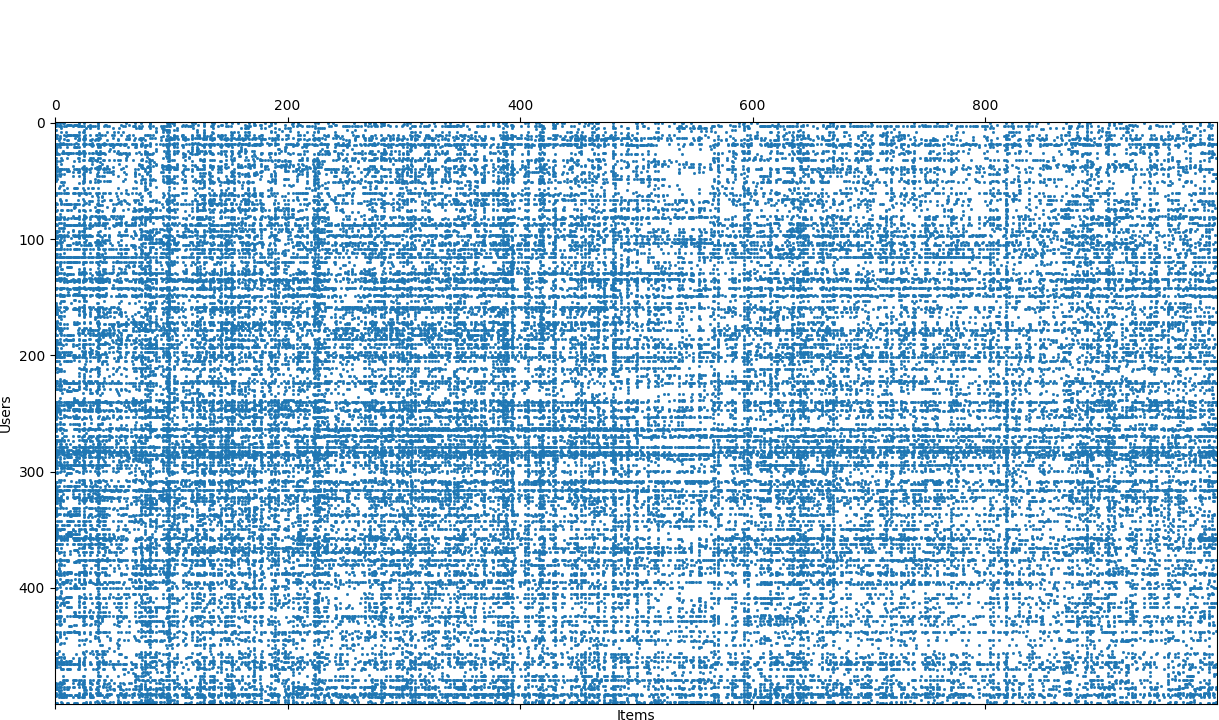
\includegraphics[width=\textwidth]{pictures/movielens-dense-target}
  \caption
  [Representation of the MovieLens 20M Dense training set.]
  {\protect\raggedright Representation of the MovieLens 20M Dense training set.}
  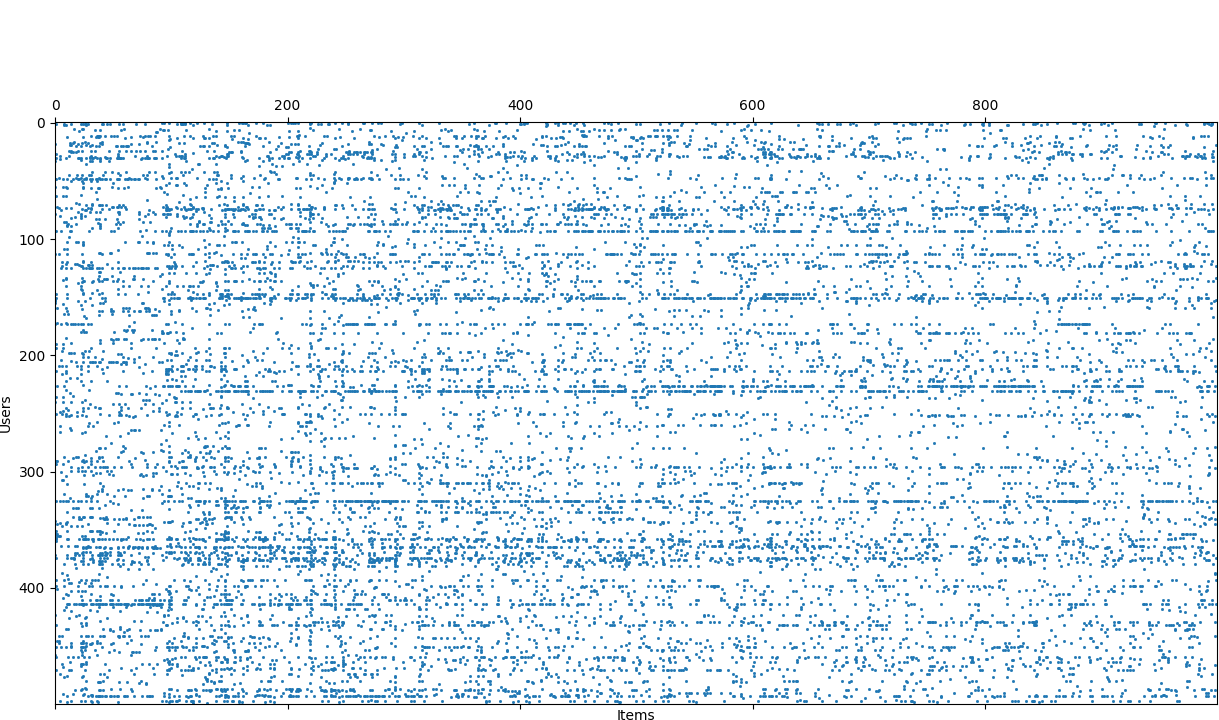
\includegraphics[width=\textwidth]{pictures/movielens-sparse-target}
  \caption
  [Representation of the MovieLens 20M Sparse training set.]
  {\protect\raggedright Representation of the MovieLens 20M Sparse training set.}
\end{figure}


\begin{table}[hbt]
\centering
\begin{tabulary}{\textwidth}{|L|CCCCCC|}
\hline
\multicolumn{7}{|c|}{MovieLens 20M $\rightarrow$ Amazon Movies TV Series (Dense)} \\
\hline
\hline
Fold 1 & mAP & nDCG & Precision & Recall & G. Div. & I. Cov. \\
\hline
TopPop & 0.0000 & 0.0000 & 0.0000 & 0.0000 & 0.0000 & 0.0000 \\
Random & 0.0000 & 0.0000 & 0.0000 & 0.0000 & 0.0000 & 0.0000 \\
kNN Prs. & 0.0000 & 0.0000 & 0.0000 & 0.0000 & 0.0000 & 0.0000 \\
kNN Cos. & 0.0000 & 0.0000 & 0.0000 & 0.0000 & 0.0000 & 0.0000 \\
rCBT Prs. & 0.0000 & 0.0000 & 0.0000 & 0.0000 & 0.0000 & 0.0000 \\
rCBT Cos. & 0.0000 & 0.0000 & 0.0000 & 0.0000 & 0.0000 & 0.0000 \\
CBT Prs. & 0.0000 & 0.0000 & 0.0000 & 0.0000 & 0.0000 & 0.0000 \\
CBT Cos. & 0.0000 & 0.0000 & 0.0000 & 0.0000 & 0.0000 & 0.0000 \\
\hline
\hline
Fold 2 & mAP & nDCG & Precision & Recall & G. Div. & I. Cov. \\
\hline
TopPop & 0.0000 & 0.0000 & 0.0000 & 0.0000 & 0.0000 & 0.0000 \\
Random & 0.0000 & 0.0000 & 0.0000 & 0.0000 & 0.0000 & 0.0000 \\
kNN Prs. & 0.0000 & 0.0000 & 0.0000 & 0.0000 & 0.0000 & 0.0000 \\
kNN Cos. & 0.0000 & 0.0000 & 0.0000 & 0.0000 & 0.0000 & 0.0000 \\
rCBT Prs. & 0.0000 & 0.0000 & 0.0000 & 0.0000 & 0.0000 & 0.0000 \\
rCBT Cos. & 0.0000 & 0.0000 & 0.0000 & 0.0000 & 0.0000 & 0.0000 \\
CBT Prs. & 0.0000 & 0.0000 & 0.0000 & 0.0000 & 0.0000 & 0.0000 \\
CBT Cos. & 0.0000 & 0.0000 & 0.0000 & 0.0000 & 0.0000 & 0.0000 \\
\hline
\hline
Fold 3 & mAP & nDCG & Precision & Recall & G. Div. & I. Cov. \\
\hline
TopPop & 0.0000 & 0.0000 & 0.0000 & 0.0000 & 0.0000 & 0.0000 \\
Random & 0.0000 & 0.0000 & 0.0000 & 0.0000 & 0.0000 & 0.0000 \\
kNN Prs. & 0.0000 & 0.0000 & 0.0000 & 0.0000 & 0.0000 & 0.0000 \\
kNN Cos. & 0.0000 & 0.0000 & 0.0000 & 0.0000 & 0.0000 & 0.0000 \\
rCBT Prs. & 0.0000 & 0.0000 & 0.0000 & 0.0000 & 0.0000 & 0.0000 \\
rCBT Cos. & 0.0000 & 0.0000 & 0.0000 & 0.0000 & 0.0000 & 0.0000 \\
CBT Prs. & 0.0000 & 0.0000 & 0.0000 & 0.0000 & 0.0000 & 0.0000 \\
CBT Cos. & 0.0000 & 0.0000 & 0.0000 & 0.0000 & 0.0000 & 0.0000 \\
\hline
\end{tabulary}
\caption{Results of CBT experiment on preprocessed target dataset for cutoff 20 on Amazon Movies TV Series (Dense), with MovieLens 20M as source domain. Higher values are better. Best results are in bold.}
\end{table}

\begin{table}[hbt]
\centering
\begin{tabulary}{\textwidth}{|L|CC|}
\hline
\multicolumn{3}{|c|}{MovieLens 20M $\rightarrow$ Amazon Movies TV Series (Dense)} \\
\hline
\hline
& mAP@20 & Difference is Significant \\
\hline
CBT Cos. & 0.0077 $\pm$ 0.0017 & \\
\hline
Random & 0.0047 $\pm$ 0.0004 & False \\
TopPop & 0.0130 $\pm$ 0.0024 & False \\
kNN Prs. & 0.0242 $\pm$ 0.0036 & True \\
kNN Cos. & 0.0476 $\pm$ 0.0060 & True \\
rCBT Prs. & 0.0094 $\pm$ 0.0015 & False \\
rCBT Cos. & 0.0078 $\pm$ 0.0011 & False \\
\hline
\hline
& mAP@20 & Difference is Significant \\
\hline
CBT Prs. & 0.0073 $\pm$ 0.0027 & \\
\hline
Random & 0.0047 $\pm$ 0.0004 & False \\
TopPop & 0.0130 $\pm$ 0.0024 & False \\
kNN Prs. & 0.0242 $\pm$ 0.0036 & False \\
kNN Cos. & 0.0476 $\pm$ 0.0060 & True \\
rCBT Prs. & 0.0094 $\pm$ 0.0015 & False \\
rCBT Cos. & 0.0078 $\pm$ 0.0011 & False \\
\hline
\end{tabulary}
\caption{Significance tests of CBT experiment on preprocessed target dataset for mAP@20 differences between CBT and baselines on Amazon Movies TV Series (Dense), with MovieLens 20M as source domain.}
\end{table}

\begin{table}[hbt]
\centering
\begin{tabulary}{\textwidth}{|L|CCCCCC|}
\hline
\multicolumn{7}{|c|}{MovieLens 20M $\rightarrow$ Amazon Movies TV Series (Sparse)} \\
\hline
\hline
Fold 1 & mAP & nDCG & Precision & Recall & G. Div. & I. Cov. \\
\hline
TopPop & 0.0000 & 0.0000 & 0.0000 & 0.0000 & 0.0000 & 0.0000 \\
Random & 0.0000 & 0.0000 & 0.0000 & 0.0000 & 0.0000 & 0.0000 \\
kNN Prs. & 0.0000 & 0.0000 & 0.0000 & 0.0000 & 0.0000 & 0.0000 \\
kNN Cos. & 0.0000 & 0.0000 & 0.0000 & 0.0000 & 0.0000 & 0.0000 \\
rCBT Prs. & 0.0000 & 0.0000 & 0.0000 & 0.0000 & 0.0000 & 0.0000 \\
rCBT Cos. & 0.0000 & 0.0000 & 0.0000 & 0.0000 & 0.0000 & 0.0000 \\
CBT Prs. & 0.0000 & 0.0000 & 0.0000 & 0.0000 & 0.0000 & 0.0000 \\
CBT Cos. & 0.0000 & 0.0000 & 0.0000 & 0.0000 & 0.0000 & 0.0000 \\
\hline
\hline
Fold 2 & mAP & nDCG & Precision & Recall & G. Div. & I. Cov. \\
\hline
TopPop & 0.0000 & 0.0000 & 0.0000 & 0.0000 & 0.0000 & 0.0000 \\
Random & 0.0000 & 0.0000 & 0.0000 & 0.0000 & 0.0000 & 0.0000 \\
kNN Prs. & 0.0000 & 0.0000 & 0.0000 & 0.0000 & 0.0000 & 0.0000 \\
kNN Cos. & 0.0000 & 0.0000 & 0.0000 & 0.0000 & 0.0000 & 0.0000 \\
rCBT Prs. & 0.0000 & 0.0000 & 0.0000 & 0.0000 & 0.0000 & 0.0000 \\
rCBT Cos. & 0.0000 & 0.0000 & 0.0000 & 0.0000 & 0.0000 & 0.0000 \\
CBT Prs. & 0.0000 & 0.0000 & 0.0000 & 0.0000 & 0.0000 & 0.0000 \\
CBT Cos. & 0.0000 & 0.0000 & 0.0000 & 0.0000 & 0.0000 & 0.0000 \\
\hline
\hline
Fold 3 & mAP & nDCG & Precision & Recall & G. Div. & I. Cov. \\
\hline
TopPop & 0.0000 & 0.0000 & 0.0000 & 0.0000 & 0.0000 & 0.0000 \\
Random & 0.0000 & 0.0000 & 0.0000 & 0.0000 & 0.0000 & 0.0000 \\
kNN Prs. & 0.0000 & 0.0000 & 0.0000 & 0.0000 & 0.0000 & 0.0000 \\
kNN Cos. & 0.0000 & 0.0000 & 0.0000 & 0.0000 & 0.0000 & 0.0000 \\
rCBT Prs. & 0.0000 & 0.0000 & 0.0000 & 0.0000 & 0.0000 & 0.0000 \\
rCBT Cos. & 0.0000 & 0.0000 & 0.0000 & 0.0000 & 0.0000 & 0.0000 \\
CBT Prs. & 0.0000 & 0.0000 & 0.0000 & 0.0000 & 0.0000 & 0.0000 \\
CBT Cos. & 0.0000 & 0.0000 & 0.0000 & 0.0000 & 0.0000 & 0.0000 \\
\hline
\end{tabulary}
\caption{Results of CBT experiment on preprocessed target dataset for cutoff 20 on Amazon Movies TV Series (Sparse), with MovieLens 20M as source domain. Higher values are better. Best results are in bold.}
\end{table}

\begin{table}[hbt]
\centering
\begin{tabulary}{\textwidth}{|L|CC|}
\hline
\multicolumn{3}{|c|}{MovieLens 20M $\rightarrow$ Amazon Movies TV Series (Sparse)} \\
\hline
\hline
& mAP@20 & Difference is Significant \\
\hline
CBT Cos. & 0.0641 $\pm$ 0.0088 & \\
\hline
Random & 0.0033 $\pm$ 0.0007 & True \\
TopPop & 0.0795 $\pm$ 0.0099 & True \\
kNN Prs. & 0.0748 $\pm$ 0.0146 & False \\
kNN Cos. & 0.0911 $\pm$ 0.0115 & True \\
rCBT Prs. & 0.0132 $\pm$ 0.0062 & True \\
rCBT Cos. & 0.0116 $\pm$ 0.0026 & True \\
\hline
\hline
& mAP@20 & Difference is Significant \\
\hline
CBT Prs. & 0.0624 $\pm$ 0.0060 & \\
\hline
Random & 0.0033 $\pm$ 0.0007 & True \\
TopPop & 0.0795 $\pm$ 0.0099 & True \\
kNN Prs. & 0.0748 $\pm$ 0.0146 & False \\
kNN Cos. & 0.0911 $\pm$ 0.0115 & True \\
rCBT Prs. & 0.0132 $\pm$ 0.0062 & True \\
rCBT Cos. & 0.0116 $\pm$ 0.0026 & True \\
\hline
\end{tabulary}
\caption{Significance tests of CBT experiment on preprocessed target dataset for mAP@20 differences between CBT and baselines on Amazon Movies TV Series (Sparse), with MovieLens 20M as source domain.}
\end{table}

\begin{table}[hbt]
\centering
\begin{tabulary}{\textwidth}{|L|CCCCCC|}
\hline
\multicolumn{7}{|c|}{MovieLens 20M $\rightarrow$ Netflix Prize (Dense)} \\
\hline
\hline
Fold 1 & mAP & nDCG & Precision & Recall & G. Div. & I. Cov. \\
\hline
TopPop & 0.0000 & 0.0000 & 0.0000 & 0.0000 & 0.0000 & 0.0000 \\
Random & 0.0000 & 0.0000 & 0.0000 & 0.0000 & 0.0000 & 0.0000 \\
kNN Prs. & 0.0000 & 0.0000 & 0.0000 & 0.0000 & 0.0000 & 0.0000 \\
kNN Cos. & 0.0000 & 0.0000 & 0.0000 & 0.0000 & 0.0000 & 0.0000 \\
rCBT Prs. & 0.0000 & 0.0000 & 0.0000 & 0.0000 & 0.0000 & 0.0000 \\
rCBT Cos. & 0.0000 & 0.0000 & 0.0000 & 0.0000 & 0.0000 & 0.0000 \\
CBT Prs. & 0.0000 & 0.0000 & 0.0000 & 0.0000 & 0.0000 & 0.0000 \\
CBT Cos. & 0.0000 & 0.0000 & 0.0000 & 0.0000 & 0.0000 & 0.0000 \\
\hline
\hline
Fold 2 & mAP & nDCG & Precision & Recall & G. Div. & I. Cov. \\
\hline
TopPop & 0.0000 & 0.0000 & 0.0000 & 0.0000 & 0.0000 & 0.0000 \\
Random & 0.0000 & 0.0000 & 0.0000 & 0.0000 & 0.0000 & 0.0000 \\
kNN Prs. & 0.0000 & 0.0000 & 0.0000 & 0.0000 & 0.0000 & 0.0000 \\
kNN Cos. & 0.0000 & 0.0000 & 0.0000 & 0.0000 & 0.0000 & 0.0000 \\
rCBT Prs. & 0.0000 & 0.0000 & 0.0000 & 0.0000 & 0.0000 & 0.0000 \\
rCBT Cos. & 0.0000 & 0.0000 & 0.0000 & 0.0000 & 0.0000 & 0.0000 \\
CBT Prs. & 0.0000 & 0.0000 & 0.0000 & 0.0000 & 0.0000 & 0.0000 \\
CBT Cos. & 0.0000 & 0.0000 & 0.0000 & 0.0000 & 0.0000 & 0.0000 \\
\hline
\hline
Fold 3 & mAP & nDCG & Precision & Recall & G. Div. & I. Cov. \\
\hline
TopPop & 0.0000 & 0.0000 & 0.0000 & 0.0000 & 0.0000 & 0.0000 \\
Random & 0.0000 & 0.0000 & 0.0000 & 0.0000 & 0.0000 & 0.0000 \\
kNN Prs. & 0.0000 & 0.0000 & 0.0000 & 0.0000 & 0.0000 & 0.0000 \\
kNN Cos. & 0.0000 & 0.0000 & 0.0000 & 0.0000 & 0.0000 & 0.0000 \\
rCBT Prs. & 0.0000 & 0.0000 & 0.0000 & 0.0000 & 0.0000 & 0.0000 \\
rCBT Cos. & 0.0000 & 0.0000 & 0.0000 & 0.0000 & 0.0000 & 0.0000 \\
CBT Prs. & 0.0000 & 0.0000 & 0.0000 & 0.0000 & 0.0000 & 0.0000 \\
CBT Cos. & 0.0000 & 0.0000 & 0.0000 & 0.0000 & 0.0000 & 0.0000 \\
\hline
\end{tabulary}
\caption{Results of CBT experiment on preprocessed target dataset for cutoff 20 on Netflix Prize (Dense), with MovieLens 20M as source domain. Higher values are better. Best results are in bold.}
\end{table}

\begin{table}[hbt]
\centering
\begin{tabulary}{\textwidth}{|L|CC|}
\hline
\multicolumn{3}{|c|}{MovieLens 20M $\rightarrow$ Netflix Prize (Dense)} \\
\hline
\hline
& mAP@20 & Difference is Significant \\
\hline
CBT Cos. & 0.0546 $\pm$ 0.0040 & \\
\hline
Random & 0.0063 $\pm$ 0.0014 & True \\
TopPop & 0.1079 $\pm$ 0.0032 & True \\
kNN Prs. & 0.1181 $\pm$ 0.0070 & True \\
kNN Cos. & 0.1573 $\pm$ 0.0101 & True \\
rCBT Prs. & 0.0599 $\pm$ 0.0045 & False \\
rCBT Cos. & 0.0588 $\pm$ 0.0048 & True \\
\hline
\hline
& mAP@20 & Difference is Significant \\
\hline
CBT Prs. & 0.0607 $\pm$ 0.0016 & \\
\hline
Random & 0.0063 $\pm$ 0.0014 & True \\
TopPop & 0.1079 $\pm$ 0.0032 & True \\
kNN Prs. & 0.1181 $\pm$ 0.0070 & True \\
kNN Cos. & 0.1573 $\pm$ 0.0101 & True \\
rCBT Prs. & 0.0599 $\pm$ 0.0045 & False \\
rCBT Cos. & 0.0588 $\pm$ 0.0048 & False \\
\hline
\end{tabulary}
\caption{Significance tests of CBT experiment on preprocessed target dataset for mAP@20 differences between CBT and baselines on Netflix Prize (Dense), with MovieLens 20M as source domain.}
\end{table}

\begin{table}[hbt]
\centering
\begin{tabulary}{\textwidth}{|L|CCCCCC|}
\hline
\multicolumn{7}{|c|}{MovieLens 20M $\rightarrow$ Netflix Prize (Sparse)} \\
\hline
\hline
Fold 1 & mAP & nDCG & Precision & Recall & G. Div. & I. Cov. \\
\hline
TopPop & 0.0000 & 0.0000 & 0.0000 & 0.0000 & 0.0000 & 0.0000 \\
Random & 0.0000 & 0.0000 & 0.0000 & 0.0000 & 0.0000 & 0.0000 \\
kNN Prs. & 0.0000 & 0.0000 & 0.0000 & 0.0000 & 0.0000 & 0.0000 \\
kNN Cos. & 0.0000 & 0.0000 & 0.0000 & 0.0000 & 0.0000 & 0.0000 \\
rCBT Prs. & 0.0000 & 0.0000 & 0.0000 & 0.0000 & 0.0000 & 0.0000 \\
rCBT Cos. & 0.0000 & 0.0000 & 0.0000 & 0.0000 & 0.0000 & 0.0000 \\
CBT Prs. & 0.0000 & 0.0000 & 0.0000 & 0.0000 & 0.0000 & 0.0000 \\
CBT Cos. & 0.0000 & 0.0000 & 0.0000 & 0.0000 & 0.0000 & 0.0000 \\
\hline
\hline
Fold 2 & mAP & nDCG & Precision & Recall & G. Div. & I. Cov. \\
\hline
TopPop & 0.0000 & 0.0000 & 0.0000 & 0.0000 & 0.0000 & 0.0000 \\
Random & 0.0000 & 0.0000 & 0.0000 & 0.0000 & 0.0000 & 0.0000 \\
kNN Prs. & 0.0000 & 0.0000 & 0.0000 & 0.0000 & 0.0000 & 0.0000 \\
kNN Cos. & 0.0000 & 0.0000 & 0.0000 & 0.0000 & 0.0000 & 0.0000 \\
rCBT Prs. & 0.0000 & 0.0000 & 0.0000 & 0.0000 & 0.0000 & 0.0000 \\
rCBT Cos. & 0.0000 & 0.0000 & 0.0000 & 0.0000 & 0.0000 & 0.0000 \\
CBT Prs. & 0.0000 & 0.0000 & 0.0000 & 0.0000 & 0.0000 & 0.0000 \\
CBT Cos. & 0.0000 & 0.0000 & 0.0000 & 0.0000 & 0.0000 & 0.0000 \\
\hline
\hline
Fold 3 & mAP & nDCG & Precision & Recall & G. Div. & I. Cov. \\
\hline
TopPop & 0.0000 & 0.0000 & 0.0000 & 0.0000 & 0.0000 & 0.0000 \\
Random & 0.0000 & 0.0000 & 0.0000 & 0.0000 & 0.0000 & 0.0000 \\
kNN Prs. & 0.0000 & 0.0000 & 0.0000 & 0.0000 & 0.0000 & 0.0000 \\
kNN Cos. & 0.0000 & 0.0000 & 0.0000 & 0.0000 & 0.0000 & 0.0000 \\
rCBT Prs. & 0.0000 & 0.0000 & 0.0000 & 0.0000 & 0.0000 & 0.0000 \\
rCBT Cos. & 0.0000 & 0.0000 & 0.0000 & 0.0000 & 0.0000 & 0.0000 \\
CBT Prs. & 0.0000 & 0.0000 & 0.0000 & 0.0000 & 0.0000 & 0.0000 \\
CBT Cos. & 0.0000 & 0.0000 & 0.0000 & 0.0000 & 0.0000 & 0.0000 \\
\hline
\end{tabulary}
\caption{Results of CBT experiment on preprocessed target dataset for cutoff 20 on Netflix Prize (Sparse), with MovieLens 20M as source domain. Higher values are better. Best results are in bold.}
\end{table}

\begin{table}[hbt]
\centering
\begin{tabulary}{\textwidth}{|L|CC|}
\hline
\multicolumn{3}{|c|}{MovieLens 20M $\rightarrow$ Netflix Prize (Sparse)} \\
\hline
\hline
& mAP@20 & Difference is Significant \\
\hline
CBT Cos. & 0.1006 $\pm$ 0.0120 & \\
\hline
Random & 0.0026 $\pm$ 0.0015 & True \\
TopPop & 0.1522 $\pm$ 0.0103 & True \\
kNN Prs. & 0.1604 $\pm$ 0.0112 & True \\
kNN Cos. & 0.1847 $\pm$ 0.0132 & True \\
rCBT Prs. & 0.1260 $\pm$ 0.0132 & True \\
rCBT Cos. & 0.1264 $\pm$ 0.0153 & True \\
\hline
\hline
& mAP@20 & Difference is Significant \\
\hline
CBT Prs. & 0.0870 $\pm$ 0.0053 & \\
\hline
Random & 0.0026 $\pm$ 0.0015 & True \\
TopPop & 0.1522 $\pm$ 0.0103 & True \\
kNN Prs. & 0.1604 $\pm$ 0.0112 & True \\
kNN Cos. & 0.1847 $\pm$ 0.0132 & True \\
rCBT Prs. & 0.1260 $\pm$ 0.0132 & True \\
rCBT Cos. & 0.1264 $\pm$ 0.0153 & True \\
\hline
\end{tabulary}
\caption{Significance tests of CBT experiment on preprocessed target dataset for mAP@20 differences between CBT and baselines on Netflix Prize (Sparse), with MovieLens 20M as source domain.}
\end{table}

\begin{table}[hbt]
\centering
\begin{tabulary}{\textwidth}{|L|CCCCCC|}
\hline
\multicolumn{7}{|c|}{Netflix Prize $\rightarrow$ Amazon Movies TV Series (Dense)} \\
\hline
\hline
Fold 1 & mAP & nDCG & Precision & Recall & G. Div. & I. Cov. \\
\hline
TopPop & 0.0000 & 0.0000 & 0.0000 & 0.0000 & 0.0000 & 0.0000 \\
Random & 0.0000 & 0.0000 & 0.0000 & 0.0000 & 0.0000 & 0.0000 \\
kNN Prs. & 0.0000 & 0.0000 & 0.0000 & 0.0000 & 0.0000 & 0.0000 \\
kNN Cos. & 0.0000 & 0.0000 & 0.0000 & 0.0000 & 0.0000 & 0.0000 \\
rCBT Prs. & 0.0000 & 0.0000 & 0.0000 & 0.0000 & 0.0000 & 0.0000 \\
rCBT Cos. & 0.0000 & 0.0000 & 0.0000 & 0.0000 & 0.0000 & 0.0000 \\
CBT Prs. & 0.0000 & 0.0000 & 0.0000 & 0.0000 & 0.0000 & 0.0000 \\
CBT Cos. & 0.0000 & 0.0000 & 0.0000 & 0.0000 & 0.0000 & 0.0000 \\
\hline
\hline
Fold 2 & mAP & nDCG & Precision & Recall & G. Div. & I. Cov. \\
\hline
TopPop & 0.0000 & 0.0000 & 0.0000 & 0.0000 & 0.0000 & 0.0000 \\
Random & 0.0000 & 0.0000 & 0.0000 & 0.0000 & 0.0000 & 0.0000 \\
kNN Prs. & 0.0000 & 0.0000 & 0.0000 & 0.0000 & 0.0000 & 0.0000 \\
kNN Cos. & 0.0000 & 0.0000 & 0.0000 & 0.0000 & 0.0000 & 0.0000 \\
rCBT Prs. & 0.0000 & 0.0000 & 0.0000 & 0.0000 & 0.0000 & 0.0000 \\
rCBT Cos. & 0.0000 & 0.0000 & 0.0000 & 0.0000 & 0.0000 & 0.0000 \\
CBT Prs. & 0.0000 & 0.0000 & 0.0000 & 0.0000 & 0.0000 & 0.0000 \\
CBT Cos. & 0.0000 & 0.0000 & 0.0000 & 0.0000 & 0.0000 & 0.0000 \\
\hline
\hline
Fold 3 & mAP & nDCG & Precision & Recall & G. Div. & I. Cov. \\
\hline
TopPop & 0.0000 & 0.0000 & 0.0000 & 0.0000 & 0.0000 & 0.0000 \\
Random & 0.0000 & 0.0000 & 0.0000 & 0.0000 & 0.0000 & 0.0000 \\
kNN Prs. & 0.0000 & 0.0000 & 0.0000 & 0.0000 & 0.0000 & 0.0000 \\
kNN Cos. & 0.0000 & 0.0000 & 0.0000 & 0.0000 & 0.0000 & 0.0000 \\
rCBT Prs. & 0.0000 & 0.0000 & 0.0000 & 0.0000 & 0.0000 & 0.0000 \\
rCBT Cos. & 0.0000 & 0.0000 & 0.0000 & 0.0000 & 0.0000 & 0.0000 \\
CBT Prs. & 0.0000 & 0.0000 & 0.0000 & 0.0000 & 0.0000 & 0.0000 \\
CBT Cos. & 0.0000 & 0.0000 & 0.0000 & 0.0000 & 0.0000 & 0.0000 \\
\hline
\end{tabulary}
\caption{Results of CBT experiment on preprocessed target dataset for cutoff 20 on Amazon Movies TV Series (Dense), with Netflix Prize as source domain. Higher values are better. Best results are in bold.}
\end{table}

\begin{table}[hbt]
\centering
\begin{tabulary}{\textwidth}{|L|CC|}
\hline
\multicolumn{3}{|c|}{Netflix Prize $\rightarrow$ Amazon Movies TV Series (Dense)} \\
\hline
\hline
& mAP@20 & Difference is Significant \\
\hline
CBT Cos. & 0.0099 $\pm$ 0.0008 & \\
\hline
Random & 0.0046 $\pm$ 0.0018 & True \\
TopPop & 0.0142 $\pm$ 0.0044 & False \\
kNN Prs. & 0.0244 $\pm$ 0.0018 & True \\
kNN Cos. & 0.0422 $\pm$ 0.0096 & True \\
rCBT Prs. & 0.0089 $\pm$ 0.0030 & False \\
rCBT Cos. & 0.0096 $\pm$ 0.0004 & False \\
\hline
\hline
& mAP@20 & Difference is Significant \\
\hline
CBT Prs. & 0.0148 $\pm$ 0.0032 & \\
\hline
Random & 0.0046 $\pm$ 0.0018 & True \\
TopPop & 0.0142 $\pm$ 0.0044 & False \\
kNN Prs. & 0.0244 $\pm$ 0.0018 & False \\
kNN Cos. & 0.0422 $\pm$ 0.0096 & True \\
rCBT Prs. & 0.0089 $\pm$ 0.0030 & False \\
rCBT Cos. & 0.0096 $\pm$ 0.0004 & False \\
\hline
\end{tabulary}
\caption{Significance tests of CBT experiment on preprocessed target dataset for mAP@20 differences between CBT and baselines on Amazon Movies TV Series (Dense), with Netflix Prize as source domain.}
\end{table}

\begin{table}[hbt]
\centering
\begin{tabulary}{\textwidth}{|L|CCCCCC|}
\hline
\multicolumn{7}{|c|}{Netflix Prize $\rightarrow$ Amazon Movies TV Series (Sparse)} \\
\hline
\hline
Fold 1 & mAP & nDCG & Precision & Recall & G. Div. & I. Cov. \\
\hline
TopPop & 0.0000 & 0.0000 & 0.0000 & 0.0000 & 0.0000 & 0.0000 \\
Random & 0.0000 & 0.0000 & 0.0000 & 0.0000 & 0.0000 & 0.0000 \\
kNN Prs. & 0.0000 & 0.0000 & 0.0000 & 0.0000 & 0.0000 & 0.0000 \\
kNN Cos. & 0.0000 & 0.0000 & 0.0000 & 0.0000 & 0.0000 & 0.0000 \\
rCBT Prs. & 0.0000 & 0.0000 & 0.0000 & 0.0000 & 0.0000 & 0.0000 \\
rCBT Cos. & 0.0000 & 0.0000 & 0.0000 & 0.0000 & 0.0000 & 0.0000 \\
CBT Prs. & 0.0000 & 0.0000 & 0.0000 & 0.0000 & 0.0000 & 0.0000 \\
CBT Cos. & 0.0000 & 0.0000 & 0.0000 & 0.0000 & 0.0000 & 0.0000 \\
\hline
\hline
Fold 2 & mAP & nDCG & Precision & Recall & G. Div. & I. Cov. \\
\hline
TopPop & 0.0000 & 0.0000 & 0.0000 & 0.0000 & 0.0000 & 0.0000 \\
Random & 0.0000 & 0.0000 & 0.0000 & 0.0000 & 0.0000 & 0.0000 \\
kNN Prs. & 0.0000 & 0.0000 & 0.0000 & 0.0000 & 0.0000 & 0.0000 \\
kNN Cos. & 0.0000 & 0.0000 & 0.0000 & 0.0000 & 0.0000 & 0.0000 \\
rCBT Prs. & 0.0000 & 0.0000 & 0.0000 & 0.0000 & 0.0000 & 0.0000 \\
rCBT Cos. & 0.0000 & 0.0000 & 0.0000 & 0.0000 & 0.0000 & 0.0000 \\
CBT Prs. & 0.0000 & 0.0000 & 0.0000 & 0.0000 & 0.0000 & 0.0000 \\
CBT Cos. & 0.0000 & 0.0000 & 0.0000 & 0.0000 & 0.0000 & 0.0000 \\
\hline
\hline
Fold 3 & mAP & nDCG & Precision & Recall & G. Div. & I. Cov. \\
\hline
TopPop & 0.0000 & 0.0000 & 0.0000 & 0.0000 & 0.0000 & 0.0000 \\
Random & 0.0000 & 0.0000 & 0.0000 & 0.0000 & 0.0000 & 0.0000 \\
kNN Prs. & 0.0000 & 0.0000 & 0.0000 & 0.0000 & 0.0000 & 0.0000 \\
kNN Cos. & 0.0000 & 0.0000 & 0.0000 & 0.0000 & 0.0000 & 0.0000 \\
rCBT Prs. & 0.0000 & 0.0000 & 0.0000 & 0.0000 & 0.0000 & 0.0000 \\
rCBT Cos. & 0.0000 & 0.0000 & 0.0000 & 0.0000 & 0.0000 & 0.0000 \\
CBT Prs. & 0.0000 & 0.0000 & 0.0000 & 0.0000 & 0.0000 & 0.0000 \\
CBT Cos. & 0.0000 & 0.0000 & 0.0000 & 0.0000 & 0.0000 & 0.0000 \\
\hline
\end{tabulary}
\caption{Results of CBT experiment on preprocessed target dataset for cutoff 20 on Amazon Movies TV Series (Sparse), with Netflix Prize as source domain. Higher values are better. Best results are in bold.}
\end{table}

\begin{table}[hbt]
\centering
\begin{tabulary}{\textwidth}{|L|CC|}
\hline
\multicolumn{3}{|c|}{Netflix Prize $\rightarrow$ Amazon Movies TV Series (Sparse)} \\
\hline
\hline
& mAP@20 & Difference is Significant \\
\hline
CBT Cos. & 0.0574 $\pm$ 0.0232 & \\
\hline
Random & 0.0047 $\pm$ 0.0015 & False \\
TopPop & 0.0922 $\pm$ 0.0131 & False \\
kNN Prs. & 0.0843 $\pm$ 0.0012 & False \\
kNN Cos. & 0.1014 $\pm$ 0.0090 & False \\
rCBT Prs. & 0.0145 $\pm$ 0.0044 & False \\
rCBT Cos. & 0.0143 $\pm$ 0.0038 & False \\
\hline
\hline
& mAP@20 & Difference is Significant \\
\hline
CBT Prs. & 0.0454 $\pm$ 0.0232 & \\
\hline
Random & 0.0047 $\pm$ 0.0015 & False \\
TopPop & 0.0922 $\pm$ 0.0131 & False \\
kNN Prs. & 0.0843 $\pm$ 0.0012 & False \\
kNN Cos. & 0.1014 $\pm$ 0.0090 & False \\
rCBT Prs. & 0.0145 $\pm$ 0.0044 & False \\
rCBT Cos. & 0.0143 $\pm$ 0.0038 & False \\
\hline
\end{tabulary}
\caption{Significance tests of CBT experiment on preprocessed target dataset for mAP@20 differences between CBT and baselines on Amazon Movies TV Series (Sparse), with Netflix Prize as source domain.}
\end{table}

\begin{table}[hbt]
\centering
\begin{tabulary}{\textwidth}{|L|CCCCCC|}
\hline
\multicolumn{7}{|c|}{Netflix Prize $\rightarrow$ MovieLens 20M (Dense)} \\
\hline
\hline
Fold 1 & mAP & nDCG & Precision & Recall & G. Div. & I. Cov. \\
\hline
TopPop & 0.0000 & 0.0000 & 0.0000 & 0.0000 & 0.0000 & 0.0000 \\
Random & 0.0000 & 0.0000 & 0.0000 & 0.0000 & 0.0000 & 0.0000 \\
kNN Prs. & 0.0000 & 0.0000 & 0.0000 & 0.0000 & 0.0000 & 0.0000 \\
kNN Cos. & 0.0000 & 0.0000 & 0.0000 & 0.0000 & 0.0000 & 0.0000 \\
rCBT Prs. & 0.0000 & 0.0000 & 0.0000 & 0.0000 & 0.0000 & 0.0000 \\
rCBT Cos. & 0.0000 & 0.0000 & 0.0000 & 0.0000 & 0.0000 & 0.0000 \\
CBT Prs. & 0.0000 & 0.0000 & 0.0000 & 0.0000 & 0.0000 & 0.0000 \\
CBT Cos. & 0.0000 & 0.0000 & 0.0000 & 0.0000 & 0.0000 & 0.0000 \\
\hline
\hline
Fold 2 & mAP & nDCG & Precision & Recall & G. Div. & I. Cov. \\
\hline
TopPop & 0.0000 & 0.0000 & 0.0000 & 0.0000 & 0.0000 & 0.0000 \\
Random & 0.0000 & 0.0000 & 0.0000 & 0.0000 & 0.0000 & 0.0000 \\
kNN Prs. & 0.0000 & 0.0000 & 0.0000 & 0.0000 & 0.0000 & 0.0000 \\
kNN Cos. & 0.0000 & 0.0000 & 0.0000 & 0.0000 & 0.0000 & 0.0000 \\
rCBT Prs. & 0.0000 & 0.0000 & 0.0000 & 0.0000 & 0.0000 & 0.0000 \\
rCBT Cos. & 0.0000 & 0.0000 & 0.0000 & 0.0000 & 0.0000 & 0.0000 \\
CBT Prs. & 0.0000 & 0.0000 & 0.0000 & 0.0000 & 0.0000 & 0.0000 \\
CBT Cos. & 0.0000 & 0.0000 & 0.0000 & 0.0000 & 0.0000 & 0.0000 \\
\hline
\hline
Fold 3 & mAP & nDCG & Precision & Recall & G. Div. & I. Cov. \\
\hline
TopPop & 0.0000 & 0.0000 & 0.0000 & 0.0000 & 0.0000 & 0.0000 \\
Random & 0.0000 & 0.0000 & 0.0000 & 0.0000 & 0.0000 & 0.0000 \\
kNN Prs. & 0.0000 & 0.0000 & 0.0000 & 0.0000 & 0.0000 & 0.0000 \\
kNN Cos. & 0.0000 & 0.0000 & 0.0000 & 0.0000 & 0.0000 & 0.0000 \\
rCBT Prs. & 0.0000 & 0.0000 & 0.0000 & 0.0000 & 0.0000 & 0.0000 \\
rCBT Cos. & 0.0000 & 0.0000 & 0.0000 & 0.0000 & 0.0000 & 0.0000 \\
CBT Prs. & 0.0000 & 0.0000 & 0.0000 & 0.0000 & 0.0000 & 0.0000 \\
CBT Cos. & 0.0000 & 0.0000 & 0.0000 & 0.0000 & 0.0000 & 0.0000 \\
\hline
\end{tabulary}
\caption{Results of CBT experiment on preprocessed target dataset for cutoff 20 on MovieLens 20M (Dense), with Netflix Prize as source domain. Higher values are better. Best results are in bold.}
\end{table}

\begin{table}[hbt]
\centering
\begin{tabulary}{\textwidth}{|L|CC|}
\hline
\multicolumn{3}{|c|}{Netflix Prize $\rightarrow$ MovieLens 20M (Dense)} \\
\hline
\hline
& mAP@20 & Difference is Significant \\
\hline
CBT Cos. & 0.0242 $\pm$ 0.0015 & \\
\hline
Random & 0.0048 $\pm$ 0.0011 & False \\
TopPop & 0.0321 $\pm$ 0.0029 & False \\
kNN Prs. & 0.0377 $\pm$ 0.0032 & False \\
kNN Cos. & 0.0576 $\pm$ 0.0062 & False \\
rCBT Prs. & 0.0230 $\pm$ 0.0058 & False \\
rCBT Cos. & 0.0247 $\pm$ 0.0011 & False \\
\hline
\hline
& mAP@20 & Difference is Significant \\
\hline
CBT Prs. & 0.0247 $\pm$ 0.0014 & \\
\hline
Random & 0.0048 $\pm$ 0.0011 & True \\
TopPop & 0.0321 $\pm$ 0.0029 & True \\
kNN Prs. & 0.0377 $\pm$ 0.0032 & True \\
kNN Cos. & 0.0576 $\pm$ 0.0062 & True \\
rCBT Prs. & 0.0230 $\pm$ 0.0058 & False \\
rCBT Cos. & 0.0247 $\pm$ 0.0011 & False \\
\hline
\end{tabulary}
\caption{Significance tests of CBT experiment on preprocessed target dataset for mAP@20 differences between CBT and baselines on MovieLens 20M (Dense), with Netflix Prize as source domain.}
\end{table}

\begin{table}[hbt]
\centering
\begin{tabulary}{\textwidth}{|L|CCCCCC|}
\hline
\multicolumn{7}{|c|}{Netflix Prize $\rightarrow$ MovieLens 20M (Sparse)} \\
\hline
\hline
Fold 1 & mAP & nDCG & Precision & Recall & G. Div. & I. Cov. \\
\hline
TopPop & 0.0000 & 0.0000 & 0.0000 & 0.0000 & 0.0000 & 0.0000 \\
Random & 0.0000 & 0.0000 & 0.0000 & 0.0000 & 0.0000 & 0.0000 \\
kNN Prs. & 0.0000 & 0.0000 & 0.0000 & 0.0000 & 0.0000 & 0.0000 \\
kNN Cos. & 0.0000 & 0.0000 & 0.0000 & 0.0000 & 0.0000 & 0.0000 \\
rCBT Prs. & 0.0000 & 0.0000 & 0.0000 & 0.0000 & 0.0000 & 0.0000 \\
rCBT Cos. & 0.0000 & 0.0000 & 0.0000 & 0.0000 & 0.0000 & 0.0000 \\
CBT Prs. & 0.0000 & 0.0000 & 0.0000 & 0.0000 & 0.0000 & 0.0000 \\
CBT Cos. & 0.0000 & 0.0000 & 0.0000 & 0.0000 & 0.0000 & 0.0000 \\
\hline
\hline
Fold 2 & mAP & nDCG & Precision & Recall & G. Div. & I. Cov. \\
\hline
TopPop & 0.0000 & 0.0000 & 0.0000 & 0.0000 & 0.0000 & 0.0000 \\
Random & 0.0000 & 0.0000 & 0.0000 & 0.0000 & 0.0000 & 0.0000 \\
kNN Prs. & 0.0000 & 0.0000 & 0.0000 & 0.0000 & 0.0000 & 0.0000 \\
kNN Cos. & 0.0000 & 0.0000 & 0.0000 & 0.0000 & 0.0000 & 0.0000 \\
rCBT Prs. & 0.0000 & 0.0000 & 0.0000 & 0.0000 & 0.0000 & 0.0000 \\
rCBT Cos. & 0.0000 & 0.0000 & 0.0000 & 0.0000 & 0.0000 & 0.0000 \\
CBT Prs. & 0.0000 & 0.0000 & 0.0000 & 0.0000 & 0.0000 & 0.0000 \\
CBT Cos. & 0.0000 & 0.0000 & 0.0000 & 0.0000 & 0.0000 & 0.0000 \\
\hline
\hline
Fold 3 & mAP & nDCG & Precision & Recall & G. Div. & I. Cov. \\
\hline
TopPop & 0.0000 & 0.0000 & 0.0000 & 0.0000 & 0.0000 & 0.0000 \\
Random & 0.0000 & 0.0000 & 0.0000 & 0.0000 & 0.0000 & 0.0000 \\
kNN Prs. & 0.0000 & 0.0000 & 0.0000 & 0.0000 & 0.0000 & 0.0000 \\
kNN Cos. & 0.0000 & 0.0000 & 0.0000 & 0.0000 & 0.0000 & 0.0000 \\
rCBT Prs. & 0.0000 & 0.0000 & 0.0000 & 0.0000 & 0.0000 & 0.0000 \\
rCBT Cos. & 0.0000 & 0.0000 & 0.0000 & 0.0000 & 0.0000 & 0.0000 \\
CBT Prs. & 0.0000 & 0.0000 & 0.0000 & 0.0000 & 0.0000 & 0.0000 \\
CBT Cos. & 0.0000 & 0.0000 & 0.0000 & 0.0000 & 0.0000 & 0.0000 \\
\hline
\end{tabulary}
\caption{Results of CBT experiment on preprocessed target dataset for cutoff 20 on MovieLens 20M (Sparse), with Netflix Prize as source domain. Higher values are better. Best results are in bold.}
\end{table}

\begin{table}[hbt]
\centering
\begin{tabulary}{\textwidth}{|L|CC|}
\hline
\multicolumn{3}{|c|}{Netflix Prize $\rightarrow$ MovieLens 20M (Sparse)} \\
\hline
\hline
& mAP@20 & Difference is Significant \\
\hline
CBT Cos. & 0.0124 $\pm$ 0.0023 & \\
\hline
Random & 0.0039 $\pm$ 0.0010 & True \\
TopPop & 0.0192 $\pm$ 0.0018 & False \\
kNN Prs. & 0.0232 $\pm$ 0.0032 & False \\
kNN Cos. & 0.0470 $\pm$ 0.0016 & True \\
rCBT Prs. & 0.0161 $\pm$ 0.0006 & False \\
rCBT Cos. & 0.0136 $\pm$ 0.0007 & False \\
\hline
\hline
& mAP@20 & Difference is Significant \\
\hline
CBT Prs. & 0.0069 $\pm$ 0.0031 & \\
\hline
Random & 0.0039 $\pm$ 0.0010 & False \\
TopPop & 0.0192 $\pm$ 0.0018 & True \\
kNN Prs. & 0.0232 $\pm$ 0.0032 & True \\
kNN Cos. & 0.0470 $\pm$ 0.0016 & True \\
rCBT Prs. & 0.0161 $\pm$ 0.0006 & False \\
rCBT Cos. & 0.0136 $\pm$ 0.0007 & False \\
\hline
\end{tabulary}
\caption{Significance tests of CBT experiment on preprocessed target dataset for mAP@20 differences between CBT and baselines on MovieLens 20M (Sparse), with Netflix Prize as source domain.}
\end{table}

\clearpage



\section{CBT: Full Target Dataset (Netflix Prize to Movielens 20M)}

The following section covers CBT experiments performed on the full Movielens 20M domain, using Netflix Prize as the source domain.\\
Experiments are run over 10 folds for each combination of source and target domains.\\
The metrics of its results are reported with a cutoff of 20.


\subsection{Datasets}

\begin{itemize}
\item \textbf{MovieLens 20M} \cite{movielens-20m-dataset}: 20 million ratings by 138,000 users on 27,000 movies, with range 1 to 5.
\item \textbf{Netflix Prize} \cite{netflix-prize-dataset}: 100,480,507 ratings by 480,189 users on 17,770 movies, with range 1 to 5.
\end{itemize}
Netflix Prize is preprocessed to extract a very dense dataset to be used as source domain.\\
Preprocessing of the source domain is performed in multiple iterations. First by removing users with a low amount of interactions. Then by removing items with a low amount of interactions. The missing ratings of the source domain are filled with the average of ratings.\\
Finally, the preprocessed and full datasets used in the experiments have the following properties:\\
\begin{center}
\begin{tabulary}{1.0\textwidth}{|L|CCCC|}
\hline
\multicolumn{5}{|c|}{Source Domain} \\
\hline
& Density & Users & Items & Ratings \\
\hline
Netflix Prize & 0 & 0 & 0 & 0 \\
\hline
\hline
\multicolumn{5}{|c|}{Target Domain} \\
\hline
& Density & Users & Items & Ratings \\
\hline
MovieLens 20M & 0 & 0 & 0 & 0 \\
\hline
\end{tabulary}
\end{center}
The target dataset is split in training and test sets. To do so, a random rating for each user is removed from the dataset and added to the test set, while the remaining ratings form the training set.


\subsection{Hyperparameters}

The hyperparameters values are estimated based on the best results of the previous experiments.\\
The following hyperparameters are set:
\begin{itemize}
\item $\texttt{construct\_validation\_every\_n} = 1$: The amount of iterations after which the codebook construction loss is evaluated by the early stopping training.
\item $\texttt{construct\_lower\_validations\_allowed} = 2000$: The amount of consecutive iterations with loss higher than the best one after which the early stopping training for codebook construction stops.
\item $\texttt{maximum\_construct\_iterations} = 20000$: The maximum amount of iterations used for codebook constructions. If the early stopping training reaches this amount, it stops.
\item $\texttt{transfer\_attempts} = 30$: The amount of attempts to find a local minimum for codebook transfer.
\item $\texttt{maximum\_fill\_iterations} = 100$: The maximum amount of iterations used to find a mapping between the target domain and the codebook. The maximum amount is the same for each of the transfer attempts.
\item $\texttt{user\_clusters} = 5$: The amount of user cluster used to build the codebook.
\item $\texttt{item\_clusters} = 5$: The amount of item cluster used to build the codebook.
\item $\texttt{knn\_topk} = 550$: The amount of similar user to consider when computing similarity for kNN.
\item $\texttt{knn\_shrink} = 120$: Shrinkage to apply when computing the similarity for kNN.
\item $\texttt{knn\_similarity} = cosine$: The similarity type to use for kNN.
\item $\texttt{knn\_normalize} = false$: Whether to normalize when computing the similarity for kNN. Normalization is computed by dividing the dot product by the product of the norms.
\end{itemize}


\begin{figure}[htb]
  \centering
  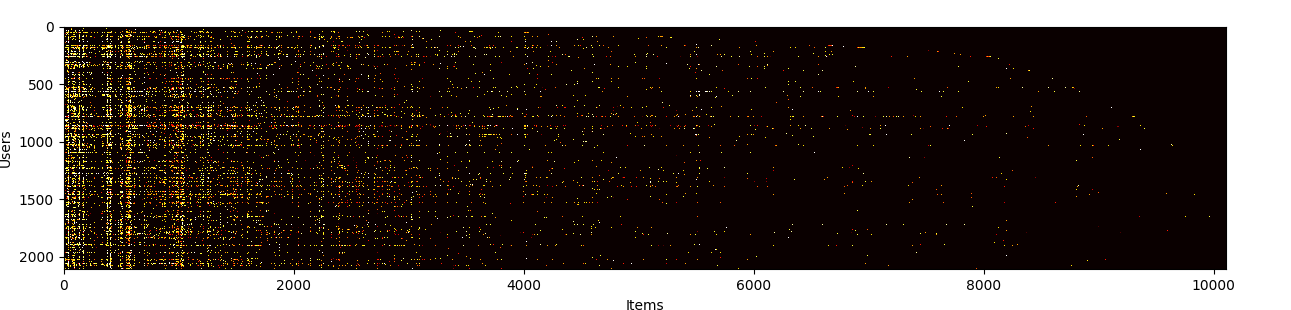
\includegraphics[width=\textwidth]{pictures/movielens-full-target}
  \caption
  [Heatmap of the MovieLens 20M original training set.]
  {\protect\raggedright Heatmap of the MovieLens 20M original training set.}
  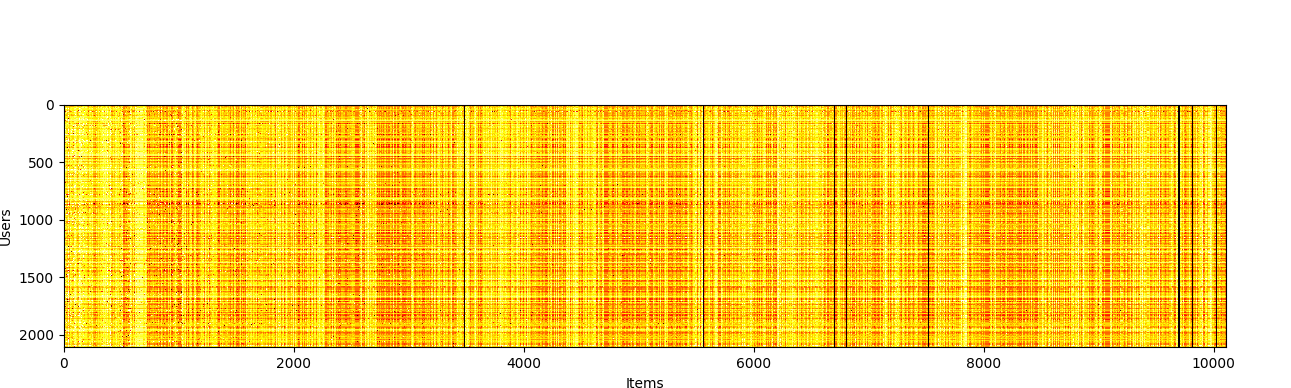
\includegraphics[width=\textwidth]{pictures/movielens-full-target-filled}
  \caption
  [Heatmap of the MovieLens 20M filled training set.]
  {\protect\raggedright Heatmap of the MovieLens 20M filled training set.}
\end{figure}


\begin{table}[hbt]
\centering
\begin{tabulary}{\textwidth}{|L|CCCCCC|}
\hline
\multicolumn{7}{|c|}{Netflix Prize $\rightarrow$ MovieLens 20M (Full)} \\
\hline
\hline
Fold 1 & mAP & nDCG & Precision & Recall & G. Div. & I. Cov. \\
\hline
TopPop & 0.0000 & 0.0000 & 0.0000 & 0.0000 & 0.0000 & 0.0000 \\
Random & 0.0000 & 0.0000 & 0.0000 & 0.0000 & 0.0000 & 0.0000 \\
kNN Cos. & 0.0000 & 0.0000 & 0.0000 & 0.0000 & 0.0000 & 0.0000 \\
CBT Cos. & 0.0000 & 0.0000 & 0.0000 & 0.0000 & 0.0000 & 0.0000 \\
\hline
\hline
Fold 2 & mAP & nDCG & Precision & Recall & G. Div. & I. Cov. \\
\hline
TopPop & 0.0000 & 0.0000 & 0.0000 & 0.0000 & 0.0000 & 0.0000 \\
Random & 0.0000 & 0.0000 & 0.0000 & 0.0000 & 0.0000 & 0.0000 \\
kNN Cos. & 0.0000 & 0.0000 & 0.0000 & 0.0000 & 0.0000 & 0.0000 \\
CBT Cos. & 0.0000 & 0.0000 & 0.0000 & 0.0000 & 0.0000 & 0.0000 \\
\hline
\hline
Fold 3 & mAP & nDCG & Precision & Recall & G. Div. & I. Cov. \\
\hline
TopPop & 0.0000 & 0.0000 & 0.0000 & 0.0000 & 0.0000 & 0.0000 \\
Random & 0.0000 & 0.0000 & 0.0000 & 0.0000 & 0.0000 & 0.0000 \\
kNN Cos. & 0.0000 & 0.0000 & 0.0000 & 0.0000 & 0.0000 & 0.0000 \\
CBT Cos. & 0.0000 & 0.0000 & 0.0000 & 0.0000 & 0.0000 & 0.0000 \\
\hline
\hline
Fold 4 & mAP & nDCG & Precision & Recall & G. Div. & I. Cov. \\
\hline
TopPop & 0.0000 & 0.0000 & 0.0000 & 0.0000 & 0.0000 & 0.0000 \\
Random & 0.0000 & 0.0000 & 0.0000 & 0.0000 & 0.0000 & 0.0000 \\
kNN Cos. & 0.0000 & 0.0000 & 0.0000 & 0.0000 & 0.0000 & 0.0000 \\
CBT Cos. & 0.0000 & 0.0000 & 0.0000 & 0.0000 & 0.0000 & 0.0000 \\
\hline
\hline
Fold 5 & mAP & nDCG & Precision & Recall & G. Div. & I. Cov. \\
\hline
TopPop & 0.0000 & 0.0000 & 0.0000 & 0.0000 & 0.0000 & 0.0000 \\
Random & 0.0000 & 0.0000 & 0.0000 & 0.0000 & 0.0000 & 0.0000 \\
kNN Cos. & 0.0000 & 0.0000 & 0.0000 & 0.0000 & 0.0000 & 0.0000 \\
CBT Cos. & 0.0000 & 0.0000 & 0.0000 & 0.0000 & 0.0000 & 0.0000 \\
\hline
\end{tabulary}
\caption{Results of CBT experiment on full target dataset for cutoff 20 on MovieLens 20M (Full), with Netflix Prize as source domain. The source domain is reduced in order to lower the sparsity. Higher values are better. Best results are in bold. Folds 1-5.}
\end{table}

\begin{table}[hbt]
\centering
\begin{tabulary}{\textwidth}{|L|CCCCCC|}
\hline
\multicolumn{7}{|c|}{Netflix Prize $\rightarrow$ MovieLens 20M (Full)} \\
\hline
\hline
Fold 6 & mAP & nDCG & Precision & Recall & G. Div. & I. Cov. \\
\hline
TopPop & 0.0000 & 0.0000 & 0.0000 & 0.0000 & 0.0000 & 0.0000 \\
Random & 0.0000 & 0.0000 & 0.0000 & 0.0000 & 0.0000 & 0.0000 \\
kNN Cos. & 0.0000 & 0.0000 & 0.0000 & 0.0000 & 0.0000 & 0.0000 \\
CBT Cos. & 0.0000 & 0.0000 & 0.0000 & 0.0000 & 0.0000 & 0.0000 \\
\hline
\hline
Fold 7 & mAP & nDCG & Precision & Recall & G. Div. & I. Cov. \\
\hline
TopPop & 0.0000 & 0.0000 & 0.0000 & 0.0000 & 0.0000 & 0.0000 \\
Random & 0.0000 & 0.0000 & 0.0000 & 0.0000 & 0.0000 & 0.0000 \\
kNN Cos. & 0.0000 & 0.0000 & 0.0000 & 0.0000 & 0.0000 & 0.0000 \\
CBT Cos. & 0.0000 & 0.0000 & 0.0000 & 0.0000 & 0.0000 & 0.0000 \\
\hline
\hline
Fold 8 & mAP & nDCG & Precision & Recall & G. Div. & I. Cov. \\
\hline
TopPop & 0.0000 & 0.0000 & 0.0000 & 0.0000 & 0.0000 & 0.0000 \\
Random & 0.0000 & 0.0000 & 0.0000 & 0.0000 & 0.0000 & 0.0000 \\
kNN Cos. & 0.0000 & 0.0000 & 0.0000 & 0.0000 & 0.0000 & 0.0000 \\
CBT Cos. & 0.0000 & 0.0000 & 0.0000 & 0.0000 & 0.0000 & 0.0000 \\
\hline
\hline
Fold 9 & mAP & nDCG & Precision & Recall & G. Div. & I. Cov. \\
\hline
TopPop & 0.0000 & 0.0000 & 0.0000 & 0.0000 & 0.0000 & 0.0000 \\
Random & 0.0000 & 0.0000 & 0.0000 & 0.0000 & 0.0000 & 0.0000 \\
kNN Cos. & 0.0000 & 0.0000 & 0.0000 & 0.0000 & 0.0000 & 0.0000 \\
CBT Cos. & 0.0000 & 0.0000 & 0.0000 & 0.0000 & 0.0000 & 0.0000 \\
\hline
\hline
Fold 10 & mAP & nDCG & Precision & Recall & G. Div. & I. Cov. \\
\hline
TopPop & 0.0000 & 0.0000 & 0.0000 & 0.0000 & 0.0000 & 0.0000 \\
Random & 0.0000 & 0.0000 & 0.0000 & 0.0000 & 0.0000 & 0.0000 \\
kNN Cos. & 0.0000 & 0.0000 & 0.0000 & 0.0000 & 0.0000 & 0.0000 \\
CBT Cos. & 0.0000 & 0.0000 & 0.0000 & 0.0000 & 0.0000 & 0.0000 \\
\hline
\end{tabulary}
\caption{Results of CBT experiment on full target dataset for cutoff 20 on MovieLens 20M (Full), with Netflix Prize as source domain. The source domain is reduced in order to lower the sparsity. Higher values are better. Best results are in bold. Folds 6-10.}
\end{table}

\begin{table}[hbt]
\centering
\begin{tabulary}{\textwidth}{|L|CC|}
\hline
\multicolumn{3}{|c|}{Netflix Prize $\rightarrow$ MovieLens 20M (Full)} \\
\hline
\hline
& mAP & Difference is Significant \\
\hline
CBT Cos. & 0.0000 $\pm$ 0.0000 & \\
\hline
Random & 0.0000 $\pm$ 0.0000 & True \\
TopPop & 0.0000 $\pm$ 0.0000 & True \\
kNN Cos. & 0.0000 $\pm$ 0.0000 & True \\
\hline
\end{tabulary}
\caption{Significance tests of CBT experiment on full target dataset for mAP@20 differences between CBT and baselines on MovieLens 20M (Full), with Netflix Prize as source domain. The source domain is reduced in order to lower the sparsity.}
\end{table}

\clearpage


\subsection{Ablation Study}

The ablation study for this experiment is performed in three different ways:
\begin{itemize}
\item \textbf{Source domain mix}: All the ratings of the source domain are shuffled without keeping rows and column relation.
\item \textbf{Random source domain}: A $500 \times 500$ source domain matrix is randomly generated with rating from 1 to 5.
\item \textbf{Source domain reduction}: One-tenth of the ratings of the source domain are removed before the source matrix is filled with the average of ratings.
\end{itemize}

\begin{table}[hbt]
\centering
\begin{tabulary}{\textwidth}{|L|CCCCCC|}
\hline
\multicolumn{7}{|c|}{Netflix Prize (Mixed) $\rightarrow$ MovieLens 20M (Full)} \\
\hline
\hline
Fold 1 & mAP & nDCG & Precision & Recall & G. Div. & I. Cov. \\
\hline
TopPop & 0.0000 & 0.0000 & 0.0000 & 0.0000 & 0.0000 & 0.0000 \\
Random & 0.0000 & 0.0000 & 0.0000 & 0.0000 & 0.0000 & 0.0000 \\
kNN Cos. & 0.0000 & 0.0000 & 0.0000 & 0.0000 & 0.0000 & 0.0000 \\
CBT Cos. & 0.0000 & 0.0000 & 0.0000 & 0.0000 & 0.0000 & 0.0000 \\
\hline
\hline
Fold 2 & mAP & nDCG & Precision & Recall & G. Div. & I. Cov. \\
\hline
TopPop & 0.0000 & 0.0000 & 0.0000 & 0.0000 & 0.0000 & 0.0000 \\
Random & 0.0000 & 0.0000 & 0.0000 & 0.0000 & 0.0000 & 0.0000 \\
kNN Cos. & 0.0000 & 0.0000 & 0.0000 & 0.0000 & 0.0000 & 0.0000 \\
CBT Cos. & 0.0000 & 0.0000 & 0.0000 & 0.0000 & 0.0000 & 0.0000 \\
\hline
\hline
Fold 3 & mAP & nDCG & Precision & Recall & G. Div. & I. Cov. \\
\hline
TopPop & 0.0000 & 0.0000 & 0.0000 & 0.0000 & 0.0000 & 0.0000 \\
Random & 0.0000 & 0.0000 & 0.0000 & 0.0000 & 0.0000 & 0.0000 \\
kNN Cos. & 0.0000 & 0.0000 & 0.0000 & 0.0000 & 0.0000 & 0.0000 \\
CBT Cos. & 0.0000 & 0.0000 & 0.0000 & 0.0000 & 0.0000 & 0.0000 \\
\hline
\hline
Fold 4 & mAP & nDCG & Precision & Recall & G. Div. & I. Cov. \\
\hline
TopPop & 0.0000 & 0.0000 & 0.0000 & 0.0000 & 0.0000 & 0.0000 \\
Random & 0.0000 & 0.0000 & 0.0000 & 0.0000 & 0.0000 & 0.0000 \\
kNN Cos. & 0.0000 & 0.0000 & 0.0000 & 0.0000 & 0.0000 & 0.0000 \\
CBT Cos. & 0.0000 & 0.0000 & 0.0000 & 0.0000 & 0.0000 & 0.0000 \\
\hline
\hline
Fold 5 & mAP & nDCG & Precision & Recall & G. Div. & I. Cov. \\
\hline
TopPop & 0.0000 & 0.0000 & 0.0000 & 0.0000 & 0.0000 & 0.0000 \\
Random & 0.0000 & 0.0000 & 0.0000 & 0.0000 & 0.0000 & 0.0000 \\
kNN Cos. & 0.0000 & 0.0000 & 0.0000 & 0.0000 & 0.0000 & 0.0000 \\
CBT Cos. & 0.0000 & 0.0000 & 0.0000 & 0.0000 & 0.0000 & 0.0000 \\
\hline
\end{tabulary}
\caption{Results of CBT experiment on full target dataset for cutoff 20 on MovieLens 20M (Full), with Netflix Prize as source domain. The source domain is reduced in order to lower the sparsity. Then, the source domain is mixed to perform the ablation study. Higher values are better. Best results are in bold. Folds 1-5.}
\end{table}

\begin{table}[hbt]
\centering
\begin{tabulary}{\textwidth}{|L|CCCCCC|}
\hline
\multicolumn{7}{|c|}{Netflix Prize (Mixed) $\rightarrow$ MovieLens 20M (Full)} \\
\hline
\hline
Fold 6 & mAP & nDCG & Precision & Recall & G. Div. & I. Cov. \\
\hline
TopPop & 0.0000 & 0.0000 & 0.0000 & 0.0000 & 0.0000 & 0.0000 \\
Random & 0.0000 & 0.0000 & 0.0000 & 0.0000 & 0.0000 & 0.0000 \\
kNN Cos. & 0.0000 & 0.0000 & 0.0000 & 0.0000 & 0.0000 & 0.0000 \\
CBT Cos. & 0.0000 & 0.0000 & 0.0000 & 0.0000 & 0.0000 & 0.0000 \\
\hline
\hline
Fold 7 & mAP & nDCG & Precision & Recall & G. Div. & I. Cov. \\
\hline
TopPop & 0.0000 & 0.0000 & 0.0000 & 0.0000 & 0.0000 & 0.0000 \\
Random & 0.0000 & 0.0000 & 0.0000 & 0.0000 & 0.0000 & 0.0000 \\
kNN Cos. & 0.0000 & 0.0000 & 0.0000 & 0.0000 & 0.0000 & 0.0000 \\
CBT Cos. & 0.0000 & 0.0000 & 0.0000 & 0.0000 & 0.0000 & 0.0000 \\
\hline
\hline
Fold 8 & mAP & nDCG & Precision & Recall & G. Div. & I. Cov. \\
\hline
TopPop & 0.0000 & 0.0000 & 0.0000 & 0.0000 & 0.0000 & 0.0000 \\
Random & 0.0000 & 0.0000 & 0.0000 & 0.0000 & 0.0000 & 0.0000 \\
kNN Cos. & 0.0000 & 0.0000 & 0.0000 & 0.0000 & 0.0000 & 0.0000 \\
CBT Cos. & 0.0000 & 0.0000 & 0.0000 & 0.0000 & 0.0000 & 0.0000 \\
\hline
\hline
Fold 9 & mAP & nDCG & Precision & Recall & G. Div. & I. Cov. \\
\hline
TopPop & 0.0000 & 0.0000 & 0.0000 & 0.0000 & 0.0000 & 0.0000 \\
Random & 0.0000 & 0.0000 & 0.0000 & 0.0000 & 0.0000 & 0.0000 \\
kNN Cos. & 0.0000 & 0.0000 & 0.0000 & 0.0000 & 0.0000 & 0.0000 \\
CBT Cos. & 0.0000 & 0.0000 & 0.0000 & 0.0000 & 0.0000 & 0.0000 \\
\hline
\hline
Fold 10 & mAP & nDCG & Precision & Recall & G. Div. & I. Cov. \\
\hline
TopPop & 0.0000 & 0.0000 & 0.0000 & 0.0000 & 0.0000 & 0.0000 \\
Random & 0.0000 & 0.0000 & 0.0000 & 0.0000 & 0.0000 & 0.0000 \\
kNN Cos. & 0.0000 & 0.0000 & 0.0000 & 0.0000 & 0.0000 & 0.0000 \\
CBT Cos. & 0.0000 & 0.0000 & 0.0000 & 0.0000 & 0.0000 & 0.0000 \\
\hline
\end{tabulary}
\caption{Results of CBT experiment on full target dataset for cutoff 20 on MovieLens 20M (Full), with Netflix Prize as source domain. The source domain is reduced in order to lower the sparsity. Then, the source domain is mixed to perform the ablation study. Higher values are better. Best results are in bold. Folds 6-10.}
\end{table}

\begin{table}[hbt]
\centering
\begin{tabulary}{\textwidth}{|L|CC|}
\hline
\multicolumn{3}{|c|}{Netflix Prize (Mixed) $\rightarrow$ MovieLens 20M (Full)} \\
\hline
\hline
& mAP & Difference is Significant \\
\hline
CBT Cos. & 0.0000 $\pm$ 0.0000 & \\
\hline
Random & 0.0000 $\pm$ 0.0000 & True \\
TopPop & 0.0000 $\pm$ 0.0000 & True \\
kNN Cos. & 0.0000 $\pm$ 0.0000 & True \\
\hline
\end{tabulary}
\caption{Significance tests of CBT experiment on full target dataset for mAP@20 differences between CBT and baselines on MovieLens 20M (Full), with Netflix Prize as source domain.  The source domain is mixed in order to lower the sparsity. Then, the source domain is mixed to perform the ablation study.}
\end{table}

\begin{table}[hbt]
\centering
\begin{tabulary}{\textwidth}{|L|CCCCCC|}
\hline
\multicolumn{7}{|c|}{Random $\rightarrow$ MovieLens 20M (Full)} \\
\hline
\hline
Fold 1 & mAP & nDCG & Precision & Recall & G. Div. & I. Cov. \\
\hline
TopPop & 0.0000 & 0.0000 & 0.0000 & 0.0000 & 0.0000 & 0.0000 \\
Random & 0.0000 & 0.0000 & 0.0000 & 0.0000 & 0.0000 & 0.0000 \\
kNN Cos. & 0.0000 & 0.0000 & 0.0000 & 0.0000 & 0.0000 & 0.0000 \\
CBT Cos. & 0.0000 & 0.0000 & 0.0000 & 0.0000 & 0.0000 & 0.0000 \\
\hline
\hline
Fold 2 & mAP & nDCG & Precision & Recall & G. Div. & I. Cov. \\
\hline
TopPop & 0.0000 & 0.0000 & 0.0000 & 0.0000 & 0.0000 & 0.0000 \\
Random & 0.0000 & 0.0000 & 0.0000 & 0.0000 & 0.0000 & 0.0000 \\
kNN Cos. & 0.0000 & 0.0000 & 0.0000 & 0.0000 & 0.0000 & 0.0000 \\
CBT Cos. & 0.0000 & 0.0000 & 0.0000 & 0.0000 & 0.0000 & 0.0000 \\
\hline
\hline
Fold 3 & mAP & nDCG & Precision & Recall & G. Div. & I. Cov. \\
\hline
TopPop & 0.0000 & 0.0000 & 0.0000 & 0.0000 & 0.0000 & 0.0000 \\
Random & 0.0000 & 0.0000 & 0.0000 & 0.0000 & 0.0000 & 0.0000 \\
kNN Cos. & 0.0000 & 0.0000 & 0.0000 & 0.0000 & 0.0000 & 0.0000 \\
CBT Cos. & 0.0000 & 0.0000 & 0.0000 & 0.0000 & 0.0000 & 0.0000 \\
\hline
\hline
Fold 4 & mAP & nDCG & Precision & Recall & G. Div. & I. Cov. \\
\hline
TopPop & 0.0000 & 0.0000 & 0.0000 & 0.0000 & 0.0000 & 0.0000 \\
Random & 0.0000 & 0.0000 & 0.0000 & 0.0000 & 0.0000 & 0.0000 \\
kNN Cos. & 0.0000 & 0.0000 & 0.0000 & 0.0000 & 0.0000 & 0.0000 \\
CBT Cos. & 0.0000 & 0.0000 & 0.0000 & 0.0000 & 0.0000 & 0.0000 \\
\hline
\hline
Fold 5 & mAP & nDCG & Precision & Recall & G. Div. & I. Cov. \\
\hline
TopPop & 0.0000 & 0.0000 & 0.0000 & 0.0000 & 0.0000 & 0.0000 \\
Random & 0.0000 & 0.0000 & 0.0000 & 0.0000 & 0.0000 & 0.0000 \\
kNN Cos. & 0.0000 & 0.0000 & 0.0000 & 0.0000 & 0.0000 & 0.0000 \\
CBT Cos. & 0.0000 & 0.0000 & 0.0000 & 0.0000 & 0.0000 & 0.0000 \\
\hline
\end{tabulary}
\caption{Results of CBT experiment on full target dataset for cutoff 20 on MovieLens 20M (Full). The source domain is randomly generated to perform the ablation study. Higher values are better. Best results are in bold. Folds 1-5.}
\end{table}

\begin{table}[hbt]
\centering
\begin{tabulary}{\textwidth}{|L|CCCCCC|}
\hline
\multicolumn{7}{|c|}{Random $\rightarrow$ MovieLens 20M (Full)} \\
\hline
\hline
Fold 6 & mAP & nDCG & Precision & Recall & G. Div. & I. Cov. \\
\hline
TopPop & 0.0000 & 0.0000 & 0.0000 & 0.0000 & 0.0000 & 0.0000 \\
Random & 0.0000 & 0.0000 & 0.0000 & 0.0000 & 0.0000 & 0.0000 \\
kNN Cos. & 0.0000 & 0.0000 & 0.0000 & 0.0000 & 0.0000 & 0.0000 \\
CBT Cos. & 0.0000 & 0.0000 & 0.0000 & 0.0000 & 0.0000 & 0.0000 \\
\hline
\hline
Fold 7 & mAP & nDCG & Precision & Recall & G. Div. & I. Cov. \\
\hline
TopPop & 0.0000 & 0.0000 & 0.0000 & 0.0000 & 0.0000 & 0.0000 \\
Random & 0.0000 & 0.0000 & 0.0000 & 0.0000 & 0.0000 & 0.0000 \\
kNN Cos. & 0.0000 & 0.0000 & 0.0000 & 0.0000 & 0.0000 & 0.0000 \\
CBT Cos. & 0.0000 & 0.0000 & 0.0000 & 0.0000 & 0.0000 & 0.0000 \\
\hline
\hline
Fold 8 & mAP & nDCG & Precision & Recall & G. Div. & I. Cov. \\
\hline
TopPop & 0.0000 & 0.0000 & 0.0000 & 0.0000 & 0.0000 & 0.0000 \\
Random & 0.0000 & 0.0000 & 0.0000 & 0.0000 & 0.0000 & 0.0000 \\
kNN Cos. & 0.0000 & 0.0000 & 0.0000 & 0.0000 & 0.0000 & 0.0000 \\
CBT Cos. & 0.0000 & 0.0000 & 0.0000 & 0.0000 & 0.0000 & 0.0000 \\
\hline
\hline
Fold 9 & mAP & nDCG & Precision & Recall & G. Div. & I. Cov. \\
\hline
TopPop & 0.0000 & 0.0000 & 0.0000 & 0.0000 & 0.0000 & 0.0000 \\
Random & 0.0000 & 0.0000 & 0.0000 & 0.0000 & 0.0000 & 0.0000 \\
kNN Cos. & 0.0000 & 0.0000 & 0.0000 & 0.0000 & 0.0000 & 0.0000 \\
CBT Cos. & 0.0000 & 0.0000 & 0.0000 & 0.0000 & 0.0000 & 0.0000 \\
\hline
\hline
Fold 10 & mAP & nDCG & Precision & Recall & G. Div. & I. Cov. \\
\hline
TopPop & 0.0000 & 0.0000 & 0.0000 & 0.0000 & 0.0000 & 0.0000 \\
Random & 0.0000 & 0.0000 & 0.0000 & 0.0000 & 0.0000 & 0.0000 \\
kNN Cos. & 0.0000 & 0.0000 & 0.0000 & 0.0000 & 0.0000 & 0.0000 \\
CBT Cos. & 0.0000 & 0.0000 & 0.0000 & 0.0000 & 0.0000 & 0.0000 \\
\hline
\end{tabulary}
\caption{Results of CBT experiment on full target dataset for cutoff 20 on MovieLens 20M (Full). The source domain is randomly generated to perform the ablation study. Higher values are better. Best results are in bold. Folds 6-10.}
\end{table}

\begin{table}[hbt]
\centering
\begin{tabulary}{\textwidth}{|L|CC|}
\hline
\multicolumn{3}{|c|}{Random $\rightarrow$ MovieLens 20M (Full)} \\
\hline
\hline
& mAP & Difference is Significant \\
\hline
CBT Cos. & 0.0000 $\pm$ 0.0000 & \\
\hline
Random & 0.0000 $\pm$ 0.0000 & True \\
TopPop & 0.0000 $\pm$ 0.0000 & True \\
kNN Cos. & 0.0000 $\pm$ 0.0000 & True \\
\hline
\end{tabulary}
\caption{Significance tests of CBT experiment on full target dataset for mAP@20 differences between CBT and baselines on MovieLens 20M (Full). The source domain is randomly generated to perform the ablation study.}
\end{table}

\begin{table}[hbt]
\centering
\begin{tabulary}{\textwidth}{|L|CCCCCC|}
\hline
\multicolumn{7}{|c|}{Netflix Prize (Removal) $\rightarrow$ MovieLens 20M (Full)} \\
\hline
\hline
Fold 1 & mAP & nDCG & Precision & Recall & G. Div. & I. Cov. \\
\hline
TopPop & 0.0000 & 0.0000 & 0.0000 & 0.0000 & 0.0000 & 0.0000 \\
Random & 0.0000 & 0.0000 & 0.0000 & 0.0000 & 0.0000 & 0.0000 \\
kNN Cos. & 0.0000 & 0.0000 & 0.0000 & 0.0000 & 0.0000 & 0.0000 \\
CBT Cos. & 0.0000 & 0.0000 & 0.0000 & 0.0000 & 0.0000 & 0.0000 \\
\hline
\hline
Fold 2 & mAP & nDCG & Precision & Recall & G. Div. & I. Cov. \\
\hline
TopPop & 0.0000 & 0.0000 & 0.0000 & 0.0000 & 0.0000 & 0.0000 \\
Random & 0.0000 & 0.0000 & 0.0000 & 0.0000 & 0.0000 & 0.0000 \\
kNN Cos. & 0.0000 & 0.0000 & 0.0000 & 0.0000 & 0.0000 & 0.0000 \\
CBT Cos. & 0.0000 & 0.0000 & 0.0000 & 0.0000 & 0.0000 & 0.0000 \\
\hline
\hline
Fold 3 & mAP & nDCG & Precision & Recall & G. Div. & I. Cov. \\
\hline
TopPop & 0.0000 & 0.0000 & 0.0000 & 0.0000 & 0.0000 & 0.0000 \\
Random & 0.0000 & 0.0000 & 0.0000 & 0.0000 & 0.0000 & 0.0000 \\
kNN Cos. & 0.0000 & 0.0000 & 0.0000 & 0.0000 & 0.0000 & 0.0000 \\
CBT Cos. & 0.0000 & 0.0000 & 0.0000 & 0.0000 & 0.0000 & 0.0000 \\
\hline
\hline
Fold 4 & mAP & nDCG & Precision & Recall & G. Div. & I. Cov. \\
\hline
TopPop & 0.0000 & 0.0000 & 0.0000 & 0.0000 & 0.0000 & 0.0000 \\
Random & 0.0000 & 0.0000 & 0.0000 & 0.0000 & 0.0000 & 0.0000 \\
kNN Cos. & 0.0000 & 0.0000 & 0.0000 & 0.0000 & 0.0000 & 0.0000 \\
CBT Cos. & 0.0000 & 0.0000 & 0.0000 & 0.0000 & 0.0000 & 0.0000 \\
\hline
\hline
Fold 5 & mAP & nDCG & Precision & Recall & G. Div. & I. Cov. \\
\hline
TopPop & 0.0000 & 0.0000 & 0.0000 & 0.0000 & 0.0000 & 0.0000 \\
Random & 0.0000 & 0.0000 & 0.0000 & 0.0000 & 0.0000 & 0.0000 \\
kNN Cos. & 0.0000 & 0.0000 & 0.0000 & 0.0000 & 0.0000 & 0.0000 \\
CBT Cos. & 0.0000 & 0.0000 & 0.0000 & 0.0000 & 0.0000 & 0.0000 \\
\hline
\end{tabulary}
\caption{Results of CBT experiment on full target dataset for cutoff 20 on MovieLens 20M (Full), with Netflix Prize as source domain. The source domain is reduced in order to lower the sparsity. Then, random ratings removal is applied to the source domain to perform the ablation study. Higher values are better. Best results are in bold. Folds 1-5.}
\end{table}

\begin{table}[hbt]
\centering
\begin{tabulary}{\textwidth}{|L|CCCCCC|}
\hline
\multicolumn{7}{|c|}{Netflix Prize (Removal) $\rightarrow$ MovieLens 20M (Full)} \\
\hline
\hline
Fold 6 & mAP & nDCG & Precision & Recall & G. Div. & I. Cov. \\
\hline
TopPop & 0.0000 & 0.0000 & 0.0000 & 0.0000 & 0.0000 & 0.0000 \\
Random & 0.0000 & 0.0000 & 0.0000 & 0.0000 & 0.0000 & 0.0000 \\
kNN Cos. & 0.0000 & 0.0000 & 0.0000 & 0.0000 & 0.0000 & 0.0000 \\
CBT Cos. & 0.0000 & 0.0000 & 0.0000 & 0.0000 & 0.0000 & 0.0000 \\
\hline
\hline
Fold 7 & mAP & nDCG & Precision & Recall & G. Div. & I. Cov. \\
\hline
TopPop & 0.0000 & 0.0000 & 0.0000 & 0.0000 & 0.0000 & 0.0000 \\
Random & 0.0000 & 0.0000 & 0.0000 & 0.0000 & 0.0000 & 0.0000 \\
kNN Cos. & 0.0000 & 0.0000 & 0.0000 & 0.0000 & 0.0000 & 0.0000 \\
CBT Cos. & 0.0000 & 0.0000 & 0.0000 & 0.0000 & 0.0000 & 0.0000 \\
\hline
\hline
Fold 8 & mAP & nDCG & Precision & Recall & G. Div. & I. Cov. \\
\hline
TopPop & 0.0000 & 0.0000 & 0.0000 & 0.0000 & 0.0000 & 0.0000 \\
Random & 0.0000 & 0.0000 & 0.0000 & 0.0000 & 0.0000 & 0.0000 \\
kNN Cos. & 0.0000 & 0.0000 & 0.0000 & 0.0000 & 0.0000 & 0.0000 \\
CBT Cos. & 0.0000 & 0.0000 & 0.0000 & 0.0000 & 0.0000 & 0.0000 \\
\hline
\hline
Fold 9 & mAP & nDCG & Precision & Recall & G. Div. & I. Cov. \\
\hline
TopPop & 0.0000 & 0.0000 & 0.0000 & 0.0000 & 0.0000 & 0.0000 \\
Random & 0.0000 & 0.0000 & 0.0000 & 0.0000 & 0.0000 & 0.0000 \\
kNN Cos. & 0.0000 & 0.0000 & 0.0000 & 0.0000 & 0.0000 & 0.0000 \\
CBT Cos. & 0.0000 & 0.0000 & 0.0000 & 0.0000 & 0.0000 & 0.0000 \\
\hline
\hline
Fold 10 & mAP & nDCG & Precision & Recall & G. Div. & I. Cov. \\
\hline
TopPop & 0.0000 & 0.0000 & 0.0000 & 0.0000 & 0.0000 & 0.0000 \\
Random & 0.0000 & 0.0000 & 0.0000 & 0.0000 & 0.0000 & 0.0000 \\
kNN Cos. & 0.0000 & 0.0000 & 0.0000 & 0.0000 & 0.0000 & 0.0000 \\
CBT Cos. & 0.0000 & 0.0000 & 0.0000 & 0.0000 & 0.0000 & 0.0000 \\
\hline
\end{tabulary}
\caption{Results of CBT experiment on full target dataset for cutoff 20 on MovieLens 20M (Full), with Netflix Prize as source domain. The source domain is reduced in order to lower the sparsity. Then, random ratings removal is applied to the source domain to perform the ablation study. Higher values are better. Best results are in bold. Folds 6-10.}
\end{table}


\begin{table}[hbt]
\centering
\begin{tabulary}{\textwidth}{|L|CC|}
\hline
\multicolumn{3}{|c|}{Netflix Prize (Removal) $\rightarrow$ MovieLens 20M (Full)} \\
\hline
\hline
& mAP & Difference is Significant \\
\hline
CBT Cos. & 0.0000 $\pm$ 0.0000 & \\
\hline
Random & 0.0000 $\pm$ 0.0000 & True \\
TopPop & 0.0000 $\pm$ 0.0000 & True \\
kNN Cos. & 0.0000 $\pm$ 0.0000 & True \\
\hline
\end{tabulary}
\caption{Significance tests of CBT experiment on full target dataset for mAP@20 differences between CBT and baselines on MovieLens 20M (Full), with Netflix Prize as source domain. The source domain is reduced in order to lower the sparsity. Then, random ratings removal is applied to the source domain to perform the ablation study.}
\end{table}

\clearpage



\section{LKT-FM: Full Target Dataset (Netflix Prize to Movielens 20M)}

The following section covers LKT-FM experiments performed on the full Movielens 20M domain, using Netflix Prize as the source domain.\\
Experiments are run over 10 folds for each combination of source and target domains.\\
The metrics of its results are reported with a cutoff of 20.


\subsection{Datasets}

\begin{itemize}
\item \textbf{MovieLens 20M} \cite{movielens-20m-dataset}: 20 million ratings by 138,000 users on 27,000 movies, with range 1 to 5.
\item \textbf{Netflix Prize} \cite{netflix-prize-dataset}: 100,480,507 ratings by 480,189 users on 17,770 movies, with range 1 to 5.
\end{itemize}
Netflix Prize is preprocessed to extract a very dense dataset to be used as source domain.\\
Preprocessing of the source domain is performed in multiple iterations. First by removing users with a low amount of interactions. Then by removing items with a low amount of interactions. The missing ratings of the source domain are filled with the average of ratings.\\
Finally, the preprocessed and full datasets used in the experiments have the following properties:\\
\begin{center}
\begin{tabulary}{1.0\textwidth}{|L|CCCC|}
\hline
\multicolumn{5}{|c|}{Source Domain} \\
\hline
& Density & Users & Items & Ratings \\
\hline
Netflix Prize & 0 & 0 & 0 & 0 \\
\hline
\hline
\multicolumn{5}{|c|}{Target Domain} \\
\hline
& Density & Users & Items & Ratings \\
\hline
MovieLens 20M & 0 & 0 & 0 & 0 \\
\hline
\end{tabulary}
\end{center}
The target dataset is split in training and test sets. To do so, a random rating for each user is removed from the dataset and added to the test set, while the remaining ratings form the training set.


\subsection{Hyperparameters}

The hyperparameters values are estimated based on the best results of the previous experiments.\\
The following hyperparameters are set:
\begin{itemize}
\item $\texttt{construct\_validation\_every\_n} = 1$: The amount of iterations after which the codebook construction loss is evaluated by the early stopping training.
\item $\texttt{construct\_lower\_validations\_allowed} = 2000$: The amount of consecutive iterations with loss higher than the best one after which the early stopping training for codebook construction stops.
\item $\texttt{maximum\_construct\_iterations} = 20000$: The maximum amount of iterations used for codebook constructions. If the early stopping training reaches this amount, it stops.
\item $\texttt{transfer\_attempts} = 30$: The amount of attempts to find a local minimum for codebook transfer.
\item $\texttt{maximum\_fill\_iterations} = 100$: The maximum amount of iterations used to find a mapping between the target domain and the codebook. The maximum amount is the same for each of the transfer attempts.
\item $\texttt{user\_clusters} = 5$: The amount of user cluster used to build the codebook.
\item $\texttt{item\_clusters} = 5$: The amount of item cluster used to build the codebook.
\item $\texttt{knn\_topk} = 550$: The amount of similar user to consider when computing similarity for kNN.
\item $\texttt{knn\_shrink} = 120$: Shrinkage to apply when computing the similarity for kNN.
\item $\texttt{knn\_similarity} = cosine$: The similarity type to use for kNN.
\item $\texttt{knn\_normalize} = false$: Whether to normalize when computing the similarity for kNN. Normalization is computed by dividing the dot product by the product of the norms.
\end{itemize}


\begin{table}[hbt]
\centering
\begin{tabulary}{\textwidth}{|L|CCCCCC|}
\hline
\multicolumn{7}{|c|}{Netflix Prize $\rightarrow$ MovieLens 20M (Full)} \\
\hline
\hline
Fold 1 & mAP & nDCG & Precision & Recall & G. Div. & I. Cov. \\
\hline
TopPop & 0.0000 & 0.0000 & 0.0000 & 0.0000 & 0.0000 & 0.0000 \\
Random & 0.0000 & 0.0000 & 0.0000 & 0.0000 & 0.0000 & 0.0000 \\
kNN Cos. & 0.0000 & 0.0000 & 0.0000 & 0.0000 & 0.0000 & 0.0000 \\
CBT Cos. & 0.0000 & 0.0000 & 0.0000 & 0.0000 & 0.0000 & 0.0000 \\
\hline
\hline
Fold 2 & mAP & nDCG & Precision & Recall & G. Div. & I. Cov. \\
\hline
TopPop & 0.0000 & 0.0000 & 0.0000 & 0.0000 & 0.0000 & 0.0000 \\
Random & 0.0000 & 0.0000 & 0.0000 & 0.0000 & 0.0000 & 0.0000 \\
kNN Cos. & 0.0000 & 0.0000 & 0.0000 & 0.0000 & 0.0000 & 0.0000 \\
CBT Cos. & 0.0000 & 0.0000 & 0.0000 & 0.0000 & 0.0000 & 0.0000 \\
\hline
\hline
Fold 3 & mAP & nDCG & Precision & Recall & G. Div. & I. Cov. \\
\hline
TopPop & 0.0000 & 0.0000 & 0.0000 & 0.0000 & 0.0000 & 0.0000 \\
Random & 0.0000 & 0.0000 & 0.0000 & 0.0000 & 0.0000 & 0.0000 \\
kNN Cos. & 0.0000 & 0.0000 & 0.0000 & 0.0000 & 0.0000 & 0.0000 \\
CBT Cos. & 0.0000 & 0.0000 & 0.0000 & 0.0000 & 0.0000 & 0.0000 \\
\hline
\hline
Fold 4 & mAP & nDCG & Precision & Recall & G. Div. & I. Cov. \\
\hline
TopPop & 0.0000 & 0.0000 & 0.0000 & 0.0000 & 0.0000 & 0.0000 \\
Random & 0.0000 & 0.0000 & 0.0000 & 0.0000 & 0.0000 & 0.0000 \\
kNN Cos. & 0.0000 & 0.0000 & 0.0000 & 0.0000 & 0.0000 & 0.0000 \\
CBT Cos. & 0.0000 & 0.0000 & 0.0000 & 0.0000 & 0.0000 & 0.0000 \\
\hline
\hline
Fold 5 & mAP & nDCG & Precision & Recall & G. Div. & I. Cov. \\
\hline
TopPop & 0.0000 & 0.0000 & 0.0000 & 0.0000 & 0.0000 & 0.0000 \\
Random & 0.0000 & 0.0000 & 0.0000 & 0.0000 & 0.0000 & 0.0000 \\
kNN Cos. & 0.0000 & 0.0000 & 0.0000 & 0.0000 & 0.0000 & 0.0000 \\
CBT Cos. & 0.0000 & 0.0000 & 0.0000 & 0.0000 & 0.0000 & 0.0000 \\
\hline
\end{tabulary}
\caption{Results of LKT-FM experiment on full target dataset for cutoff 20 on MovieLens 20M (Full), with Netflix Prize as source domain. The source domain is reduced in order to lower the sparsity. Higher values are better. Best results are in bold. Folds 1-5.}
\end{table}

\begin{table}[hbt]
\centering
\begin{tabulary}{\textwidth}{|L|CCCCCC|}
\hline
\multicolumn{7}{|c|}{Netflix Prize $\rightarrow$ MovieLens 20M (Full)} \\
\hline
\hline
Fold 6 & mAP & nDCG & Precision & Recall & G. Div. & I. Cov. \\
\hline
TopPop & 0.0000 & 0.0000 & 0.0000 & 0.0000 & 0.0000 & 0.0000 \\
Random & 0.0000 & 0.0000 & 0.0000 & 0.0000 & 0.0000 & 0.0000 \\
kNN Cos. & 0.0000 & 0.0000 & 0.0000 & 0.0000 & 0.0000 & 0.0000 \\
CBT Cos. & 0.0000 & 0.0000 & 0.0000 & 0.0000 & 0.0000 & 0.0000 \\
\hline
\hline
Fold 7 & mAP & nDCG & Precision & Recall & G. Div. & I. Cov. \\
\hline
TopPop & 0.0000 & 0.0000 & 0.0000 & 0.0000 & 0.0000 & 0.0000 \\
Random & 0.0000 & 0.0000 & 0.0000 & 0.0000 & 0.0000 & 0.0000 \\
kNN Cos. & 0.0000 & 0.0000 & 0.0000 & 0.0000 & 0.0000 & 0.0000 \\
CBT Cos. & 0.0000 & 0.0000 & 0.0000 & 0.0000 & 0.0000 & 0.0000 \\
\hline
\hline
Fold 8 & mAP & nDCG & Precision & Recall & G. Div. & I. Cov. \\
\hline
TopPop & 0.0000 & 0.0000 & 0.0000 & 0.0000 & 0.0000 & 0.0000 \\
Random & 0.0000 & 0.0000 & 0.0000 & 0.0000 & 0.0000 & 0.0000 \\
kNN Cos. & 0.0000 & 0.0000 & 0.0000 & 0.0000 & 0.0000 & 0.0000 \\
CBT Cos. & 0.0000 & 0.0000 & 0.0000 & 0.0000 & 0.0000 & 0.0000 \\
\hline
\hline
Fold 9 & mAP & nDCG & Precision & Recall & G. Div. & I. Cov. \\
\hline
TopPop & 0.0000 & 0.0000 & 0.0000 & 0.0000 & 0.0000 & 0.0000 \\
Random & 0.0000 & 0.0000 & 0.0000 & 0.0000 & 0.0000 & 0.0000 \\
kNN Cos. & 0.0000 & 0.0000 & 0.0000 & 0.0000 & 0.0000 & 0.0000 \\
CBT Cos. & 0.0000 & 0.0000 & 0.0000 & 0.0000 & 0.0000 & 0.0000 \\
\hline
\hline
Fold 10 & mAP & nDCG & Precision & Recall & G. Div. & I. Cov. \\
\hline
TopPop & 0.0000 & 0.0000 & 0.0000 & 0.0000 & 0.0000 & 0.0000 \\
Random & 0.0000 & 0.0000 & 0.0000 & 0.0000 & 0.0000 & 0.0000 \\
kNN Cos. & 0.0000 & 0.0000 & 0.0000 & 0.0000 & 0.0000 & 0.0000 \\
CBT Cos. & 0.0000 & 0.0000 & 0.0000 & 0.0000 & 0.0000 & 0.0000 \\
\hline
\end{tabulary}
\caption{Results of LKT-FM experiment on full target dataset for cutoff 20 on MovieLens 20M (Full), with Netflix Prize as source domain. The source domain is reduced in order to lower the sparsity. Higher values are better. Best results are in bold. Folds 6-10.}
\end{table}

\begin{table}[hbt]
\centering
\begin{tabulary}{\textwidth}{|L|CC|}
\hline
\multicolumn{3}{|c|}{Netflix Prize $\rightarrow$ MovieLens 20M (Full)} \\
\hline
\hline
& mAP & Difference is Significant \\
\hline
LKT-FM Cos. & 0.0015 $\pm$ 0.0009 & \\
\hline
Random & 0.0004 $\pm$ 0.0003 & True \\
TopPop & 0.0489 $\pm$ 0.0041 & True \\
kNN Cos. & 0.0672 $\pm$ 0.0027 & True \\
\hline
\end{tabulary}
\caption{Significance tests of LKT-FM experiment on full target dataset for mAP@20 differences between LKT-FM and baselines on MovieLens 20M (Full), with Netflix Prize as source domain. The source domain is reduced in order to lower the sparsity.}
\end{table}
